\documentclass[12pt]{report}
\usepackage{../mystyle}
\begin{document}
\boldmath
\fancyhead[L]{Homework 5}
\fancyhead[C]{Ordered sets in Data Analysis}
\fancyhead[R]{Ryabykin Aleksey}
\begin{problem}{}
    Consider the Wheel Chains Dataset (Table \ref{table:data}) we encountered in the lectures. In this task we will consider any system which had a grade above $2.3$ an accepted system, otherwise it is unacceeted.
    \begin{table}[H]
        \centering
        \begin{tabular}{|c|c|c|c|c|c|c|c|c|}
        \hline
        N\textsuperscript{\underline{o}}  & System & mount  & price & con & snow & ice & dur & Accegrade \\ \hline
        1  & SK     & F      & 206   & 1.9 & 1.4  & 1.8 & 2.7 & F         \\ \hline
        2  & SRK    & F or R & 520   & 2.1 & 0.8  & 3.8 & 2.3 & F         \\ \hline
        3  & SK     & F      & 160   & 1.7 & 1.9  & 1.6 & 3.7 & F         \\ \hline
        4  & SK     & F      & 213   & 1.7 & 2.0  & 2.4 & 3.4 & F         \\ \hline
        5  & SMS    & F or R & 598   & 1.6 & 2.4  & 7   & 2.8 & F         \\ \hline
        6  & SK     & F      & 109   & 2.0 & 1.9  & 2.4 & 3.7 & F         \\ \hline
        7  & SRK    & F or R & 325   & 2.0 & 2.1  & 3.2 & 2.8 & F         \\ \hline
        8  & SMS    & F or R & 498   & 1.5 & 3.3  & 3.5 & 2.0 & T         \\ \hline
        9  & SRK    & F or R & 396   & 2.8 & 2.1  & 3.1 & 2.5 & T         \\ \hline
        10 & SRK    & F or R & 325   & 2.2 & 2.2  & 4.6 & 3.2 & T         \\ \hline
        11 & SRK    & F or R & 389   & 2.0 & 2.2  & 3.3 & 4.3 & T         \\ \hline
        12 & SRK    & F      & 298   & 2.5 & 2.3  & 3.3 & 2.8 & T         \\ \hline
        13 & SK     & F      & 149   & 1.9 & 2.5  & 4.0 & 3.8 & T         \\ \hline
        14 & SMS    & F or R & 684   & 1.7 & 3.3  & 4.4 & 2.2 & T         \\ \hline
        15 & SK     & F      & 99    & 2.8 & 2.2  & 2.5 & 4.0 & T         \\ \hline
        16 & SK     & F      & 140   & 2.6 & 2.3  & 3.3 & 3.4 & T         \\ \hline
        17 & SK     & F      & 215   & 2.3 & 3.8  & 4.8 & 2.3 & T         \\ \hline
        \end{tabular}
    \caption{Wheel Chains Dataset with initial order}
    \label{table:data}
    \end{table}
    \begin{enumerate}
        \item Consider the last three examples of this dataset only (no cross validation) and classify them using lazy classification with pattern structures (with interval pattern structures for numerical attributes). What is the accuracy of this classification? Why do you think that happend?
        \item Now let's consider the same dataset, with a different order (Table \ref{table:data_order}) below. Try to classify same three examples, what is the accuracy?

    \begin{table}
        \centering
\begin{tabular}{|c|c|c|c|c|c|c|c|c|}
\hline
N\textsuperscript{\underline{o}}  & System & mount  & price & con & snow & ice & dur & Accegrade \\ \hline
1  & SK     & F      & 149   & 1.9 & 2.5  & 4.0 & 3.8 & T         \\ \hline
2  & SRK    & F or R & 520   & 2.1 & 0.8  & 3.8 & 2.3 & F         \\ \hline
3  & SRK    & F or R & 389   & 2.0 & 2.2  & 3.3 & 4.3 & T         \\ \hline
4  & SK     & F      & 213   & 1.7 & 2.0  & 2.4 & 3.4 & F         \\ \hline
5  & SMS    & F or R & 598   & 1.6 & 2.4  & 7   & 2.8 & F         \\ \hline
6  & SK     & F      & 109   & 2.0 & 1.9  & 2.4 & 3.7 & F         \\ \hline
7  & SRK    & F or R & 325   & 2.0 & 2.1  & 3.2 & 2.8 & F         \\ \hline
8  & SMS    & F or R & 498   & 1.5 & 3.3  & 3.5 & 2.0 & T         \\ \hline
9  & SRK    & F or R & 396   & 2.8 & 2.1  & 3.1 & 2.5 & T         \\ \hline
10 & SK     & F      & 160   & 1.7 & 1.9  & 1.6 & 3.7 & F         \\ \hline
11 & SRK    & F or R & 325   & 2.2 & 2.2  & 4.6 & 3.2 & T         \\ \hline
12 & SRK    & F      & 298   & 2.5 & 2.3  & 3.3 & 2.8 & T         \\ \hline
13 & SK     & F      & 206   & 1.9 & 1.4  & 1.8 & 2.7 & F         \\ \hline
14 & SMS    & F or R & 684   & 1.7 & 3.3  & 4.4 & 2.2 & T         \\ \hline
15 & SK     & F      & 99    & 2.8 & 2.2  & 2.5 & 4.0 & T         \\ \hline
16 & SK     & F      & 140   & 2.6 & 2.3  & 3.3 & 3.4 & T         \\ \hline
17 & SK     & F      & 215   & 2.3 & 3.8  & 4.8 & 2.3 & T         \\ \hline
\end{tabular}
\caption{Dataset with different ordering}
\label{table:data_order}
\end{table}
    \item Assess the performance of the lazy classification with interval pattern structures on the randomly ordered sample (the second one) by applying 5-cross validation.
    \item We define a new type of interval pattern structures as follows:
    \par 
    IF the value of attribute $J$ for object $I$ is $w(I, J)$, the value of the pattern structure will be: $[w(I, J), \infty]$. We will also define the intersection on such intervals as:
    \[
        [a_1, \infty] \cap [a_2, \infty] = [\min (a_1, a_2), \infty].  
    \]
    Classify the example number 15 using the newly defined pattern structures.
    \item We define a new type of interval pattern structures as follows:
    \par 
    If the value of attribute $J$ for object $I$ is $w(I, J)$, the value of the pattern structure will be: $[w(I,J), \infty]$. We will also define the intersection on such intervals as:
    \[
        [a_1, \infty] \cap [a_2, \infty] = [\max (a_1, a_2), \infty]  
    \]
    Classify the example number 15 using the newly define pattern structures. Which one of the defined interval pattern structures is most suitable for our dataset? Why?
    \end{enumerate}
\end{problem}
\begin{solution}
    \begin{enumerate}
        \item Pattern structures used here:
        \begin{itemize}
            \item For the nominal attributes, we will use the set theoric intersection;
            \item For the numerical attributes, we will use the interval pattern structures, where we replace the attribute value $w(I,J)$ where $I$ is the object and $J$ is the attribute, with an interval $[w(I, J), w(I,J)]$
        \end{itemize}
        Let me take the last three examples of the dataset:
        \begin{table}[H]
            \centering
            \begin{tabular}{|c|c|c|c|c|c|c|c|c|}
            \hline
            N\textsuperscript{\underline{o}}  & System & mount & price & con & snow & ice & dur & Accegrade \\ \hline
            15 & SK     & F     & 99    & 2.8  & 2.2  & 2.5 & 4.0 & T         \\ \hline
            16 & SK     & F     & 140   & 2.6 & 2.3  & 3.3 & 3.4 & T         \\ \hline
            17 & SK     & F     & 215   & 2.3 & 3.8  & 4.8 & 2.3 & T         \\ \hline
            \end{tabular}
            \end{table}
        \subsubsection*{The first test example:}
        \par 
        we will loop through all objects in the training dataset and repeat these next steps until we reach a classification:
        \begin{itemize}
            \item We compute: $\text{IntSec} = \delta (g) \cap \delta (g_t) = \langle SK, F, [99, 206], [1.9, 2.8], [1.4, 2.2], [1.8, 2.5], [2.7, 4.0] \rangle.$
            \item Now we compute the extension $\text{Ext} = \left(\text{IntSec}\right)'$ (Table \ref{table:ext1}):
            \[
                \text{Ext} = \langle 1, 6\rangle.
            \]
            They are both False, then we classify the first object as False.
        \end{itemize}
        \begin{table}[H]
            \centering
            \begin{tabular}{|c|c|c|c|c|c|c|c|c|}
            \hline
            N\textsuperscript{\underline{o}} &
              System &
              mount &
              price &
              con &
              snow &
              ice &
              dur &
              Accegrade \\ \hline
            \rowcolor[HTML]{34FF34} 
            1 &
              SK &
              F &
              206 &
              1.9 &
              1.4 &
              1.8 &
              2.7 &
              F \\ \hline
            2 &
              \cellcolor[HTML]{FE0000}SRK &
              \cellcolor[HTML]{FFFFFF}F or R &
              520 &
              2.1 &
              0.8 &
              3.8 &
              2.3 &
              F \\ \hline
            3 &
              SK &
              F &
              160 &
              \cellcolor[HTML]{FE0000}1.7 &
              1.9 &
              1.6 &
              3.7 &
              F \\ \hline
            4 &
              SK &
              F &
              \cellcolor[HTML]{FE0000}213 &
              1.7 &
              2.0 &
              2.4 &
              3.4 &
              F \\ \hline
            5 &
              \cellcolor[HTML]{FE0000}SMS &
              F or R &
              \cellcolor[HTML]{FFFFFF}598 &
              1.6 &
              2.4 &
              7 &
              2.8 &
              F \\ \hline
            \rowcolor[HTML]{34FF34} 
            6 &
              SK &
              F &
              109 &
              2.0 &
              1.9 &
              2.4 &
              3.7 &
              F \\ \hline
            7 &
              \cellcolor[HTML]{FE0000}SRK &
              F or R &
              325 &
              2.0 &
              2.1 &
              3.2 &
              2.8 &
              F \\ \hline
            8 &
              \cellcolor[HTML]{FE0000}SMS &
              F or R &
              498 &
              1.5 &
              3.3 &
              3.5 &
              2.0 &
              T \\ \hline
            9 &
              \cellcolor[HTML]{FE0000}SRK &
              F or R &
              396 &
              2.8 &
              2.1 &
              3.1 &
              2.5 &
              T \\ \hline
            10 &
              \cellcolor[HTML]{FE0000}SRK &
              F or R &
              325 &
              2.2 &
              2.2 &
              4.6 &
              3.2 &
              T \\ \hline
            11 &
              \cellcolor[HTML]{FE0000}SRK &
              F or R &
              389 &
              2.0 &
              2.2 &
              3.3 &
              4.3 &
              T \\ \hline
            12 &
              \cellcolor[HTML]{FE0000}SRK &
              F &
              298 &
              2.5 &
              2.3 &
              3.3 &
              2.8 &
              T \\ \hline
            13 &
              SK &
              F &
              149 &
              1.9 &
              \cellcolor[HTML]{FE0000}2.5 &
              4.0 &
              3.8 &
              T \\ \hline
            14 &
              \cellcolor[HTML]{FE0000}SMS &
              F or R &
              684 &
              1.7 &
              3.3 &
              4.4 &
              2.2 &
              T \\ \hline
            \end{tabular}
            \caption{Extension for first test example}
            \label{table:ext1}
            \end{table}
        \subsubsection*{The second test example}
        Let's apply the same algorithm to the second test example:
        \begin{itemize}
            \item $\text{IntSec} = \langle SK, F, [140, 206], [1.9, 2.6], [1.4,2.3], [1.8, 3.3], [2.7, 3.4]\rangle$
            \item $\text{Ext} = (\text{IntSec})'$ (Table \ref{table:ext2}):
            \begin{table}[H]
                \centering
                \begin{tabular}{|c|c|c|c|c|c|c|c|c|}
                \hline
                N\textsuperscript{\underline{o}} &
                  System &
                  mount &
                  price &
                  con &
                  snow &
                  ice &
                  dur &
                  Accegrade \\ \hline
                \rowcolor[HTML]{34FF34} 
                1 &
                  SK &
                  F &
                  206 &
                  1.9 &
                  1.4 &
                  1.8 &
                  2.7 &
                  F \\ \hline
                2 &
                  \cellcolor[HTML]{FE0000}SRK &
                  \cellcolor[HTML]{FFFFFF}F or R &
                  520 &
                  2.1 &
                  0.8 &
                  3.8 &
                  2.3 &
                  F \\ \hline
                3 &
                  SK &
                  F &
                  160 &
                  \cellcolor[HTML]{FE0000}1.7 &
                  1.9 &
                  1.6 &
                  3.7 &
                  F \\ \hline
                4 &
                  SK &
                  F &
                  \cellcolor[HTML]{FE0000}213 &
                  1.7 &
                  2.0 &
                  2.4 &
                  3.4 &
                  F \\ \hline
                5 &
                  \cellcolor[HTML]{FE0000}SMS &
                  F or R &
                  \cellcolor[HTML]{FFFFFF}598 &
                  1.6 &
                  2.4 &
                  7 &
                  2.8 &
                  F \\ \hline
                \rowcolor[HTML]{FFFFFF} 
                6 &
                  SK &
                  F &
                  109 &
                  2.0 &
                  1.9 &
                  2.4 &
                  \cellcolor[HTML]{FE0000}3.7 &
                  F \\ \hline
                7 &
                  \cellcolor[HTML]{FE0000}SRK &
                  F or R &
                  325 &
                  2.0 &
                  2.1 &
                  3.2 &
                  2.8 &
                  F \\ \hline
                8 &
                  \cellcolor[HTML]{FE0000}SMS &
                  F or R &
                  498 &
                  1.5 &
                  3.3 &
                  3.5 &
                  2.0 &
                  T \\ \hline
                9 &
                  \cellcolor[HTML]{FE0000}SRK &
                  F or R &
                  396 &
                  2.8 &
                  2.1 &
                  3.1 &
                  2.5 &
                  T \\ \hline
                10 &
                  \cellcolor[HTML]{FE0000}SRK &
                  F or R &
                  325 &
                  2.2 &
                  2.2 &
                  4.6 &
                  3.2 &
                  T \\ \hline
                11 &
                  \cellcolor[HTML]{FE0000}SRK &
                  F or R &
                  389 &
                  2.0 &
                  2.2 &
                  3.3 &
                  4.3 &
                  T \\ \hline
                12 &
                  \cellcolor[HTML]{FE0000}SRK &
                  F &
                  298 &
                  2.5 &
                  2.3 &
                  3.3 &
                  2.8 &
                  T \\ \hline
                13 &
                  SK &
                  F &
                  149 &
                  1.9 &
                  \cellcolor[HTML]{FFFFFF}2.5 &
                  \cellcolor[HTML]{FE0000}4.0 &
                  3.8 &
                  T \\ \hline
                14 &
                  \cellcolor[HTML]{FE0000}SMS &
                  F or R &
                  684 &
                  1.7 &
                  3.3 &
                  4.4 &
                  2.2 &
                  T \\ \hline
                \end{tabular}
                \caption{Extension for the second test example}
                \label{table:ext2}
                \end{table}
                So, we notice that all of them are False, then we classify our example with the same value.
        \end{itemize}
        \subsubsection*{The third test example}
        Same for the last one in the test set:
        \begin{itemize}
            \item $\text{IntSec} = \langle SK, F, [206, 215], [1.9, 2.3], [1.4, 3.8], [1.8, 4.8], [2.3, 2.7]\rangle$
            \item $\text{Ext} = (\text{IntSec})'$ (Table \ref{table:ext3})
            \begin{table}[H]
                \centering
                \begin{tabular}{|c|c|c|c|c|c|c|c|c|}
                \hline
                N\textsuperscript{\underline{o}} & System                      & mount  & price                       & con                         & snow & ice & dur & Accegrade \\ \hline
                \rowcolor[HTML]{34FF34} 
                1  & SK                          & F      & 206                         & 1.9                         & 1.4  & 1.8 & 2.7 & F         \\ \hline
                2 &
                  \cellcolor[HTML]{FE0000}SRK &
                  \cellcolor[HTML]{FFFFFF}F or R &
                  520 &
                  2.1 &
                  0.8 &
                  3.8 &
                  2.3 &
                  F \\ \hline
                3  & SK                          & F      & \cellcolor[HTML]{FE0000}160 & \cellcolor[HTML]{FFFFFF}1.7 & 1.9  & 1.6 & 3.7 & F         \\ \hline
                4  & SK                          & F      & \cellcolor[HTML]{FFFFFF}213 & \cellcolor[HTML]{FE0000}1.7 & 2.0  & 2.4 & 3.4 & F         \\ \hline
                5 &
                  \cellcolor[HTML]{FE0000}SMS &
                  F or R &
                  \cellcolor[HTML]{FFFFFF}598 &
                  1.6 &
                  2.4 &
                  7 &
                  2.8 &
                  F \\ \hline
                \rowcolor[HTML]{FFFFFF} 
                6  & SK                          & F      & \cellcolor[HTML]{FE0000}109 & 2.0                         & 1.9  & 2.4 & 3.7 & F         \\ \hline
                7  & \cellcolor[HTML]{FE0000}SRK & F or R & 325                         & 2.0                         & 2.1  & 3.2 & 2.8 & F         \\ \hline
                8  & \cellcolor[HTML]{FE0000}SMS & F or R & 498                         & 1.5                         & 3.3  & 3.5 & 2.0 & T         \\ \hline
                9  & \cellcolor[HTML]{FE0000}SRK & F or R & 396                         & 2.8                         & 2.1  & 3.1 & 2.5 & T         \\ \hline
                10 & \cellcolor[HTML]{FE0000}SRK & F or R & 325                         & 2.2                         & 2.2  & 4.6 & 3.2 & T         \\ \hline
                11 & \cellcolor[HTML]{FE0000}SRK & F or R & 389                         & 2.0                         & 2.2  & 3.3 & 4.3 & T         \\ \hline
                12 & \cellcolor[HTML]{FE0000}SRK & F      & 298                         & 2.5                         & 2.3  & 3.3 & 2.8 & T         \\ \hline
                13 &
                  SK &
                  F &
                  \cellcolor[HTML]{FE0000}149 &
                  1.9 &
                  \cellcolor[HTML]{FFFFFF}2.5 &
                  \cellcolor[HTML]{FFFFFF}4.0 &
                  3.8 &
                  T \\ \hline
                14 & \cellcolor[HTML]{FE0000}SMS & F or R & 684                         & 1.7                         & 3.3  & 4.4 & 2.2 & T         \\ \hline
                \end{tabular}
                \caption{Extension for the third test example}
                \label{table:ext3}
                \end{table}
            The same as for the second test example. We predict False value of the target variable. 
        \end{itemize}
        \par
            Inferences: our final accuracy is $0\%$. It became real because of the inital data ordering.
            \item Let's do the same for the data with another ordering (Table \ref{table:data_order}):
            \vspace*{-0.3cm}
            
            \subsubsection*{The first test example}
            \begin{itemize}
              \item $\text{IntSec} = \langle SK, F, [99, 149], [1.9, 2.8], [2.2, 2.5], [2.5, 4.0], [3.8, 4.0]\rangle$
              \item The extension (Table \ref{table:ext1_1}):
              \useshortskip
              \[
                  \text{Ext} = \langle 1\rangle
              \]
              \useshortskip
              We predict True value for the target variable.
              \vspace*{-0.3cm}

              \begin{table}[H]
                \centering
                \begin{tabular}{|c|c|c|c|c|c|c|c|c|}
                \hline
                N\textsuperscript{\underline{o}} & System                      & mount  & price                       & con & snow                        & ice & dur & Accegrade \\ \hline
                \rowcolor[HTML]{34FF34} 
                1  & SK                          & F      & 149                         & 1.9 & 2.5                         & 4.0 & 3.8 & T         \\ \hline
                2  & \cellcolor[HTML]{FE0000}SRK & F or R & 520                         & 2.1 & 0.8                         & 3.8 & 2.3 & F         \\ \hline
                3  & \cellcolor[HTML]{FE0000}SRK & F or R & 389                         & 2.0 & 2.2                         & 3.3 & 4.3 & T         \\ \hline
                4  & SK                          & F      & \cellcolor[HTML]{FE0000}213 & 1.7 & 2.0                         & 2.4 & 3.4 & F         \\ \hline
                5  & \cellcolor[HTML]{FE0000}SMS & F or R & 598                         & 1.6 & 2.4                         & 7   & 2.8 & F         \\ \hline
                6  & SK                          & F      & 109                         & 2.0 & \cellcolor[HTML]{FE0000}1.9 & 2.4 & 3.7 & F         \\ \hline
                7  & \cellcolor[HTML]{FE0000}SRK & F or R & 325                         & 2.0 & 2.1                         & 3.2 & 2.8 & F         \\ \hline
                8  & \cellcolor[HTML]{FE0000}SMS & F or R & 498                         & 1.5 & 3.3                         & 3.5 & 2.0 & T         \\ \hline
                9  & \cellcolor[HTML]{FE0000}SRK & F or R & 396                         & 2.8 & 2.1                         & 3.1 & 2.5 & T         \\ \hline
                10 & SK                          & F      & \cellcolor[HTML]{FE0000}160 & 1.7 & 1.9                         & 1.6 & 3.7 & F         \\ \hline
                11 & \cellcolor[HTML]{FE0000}SRK & F or R & 325                         & 2.2 & 2.2                         & 4.6 & 3.2 & T         \\ \hline
                12 & \cellcolor[HTML]{FE0000}SRK & F      & 298                         & 2.5 & 2.3                         & 3.3 & 2.8 & T         \\ \hline
                13 & SK                          & F      & \cellcolor[HTML]{FE0000}206 & 1.9 & 1.4                         & 1.8 & 2.7 & F         \\ \hline
                14 & \cellcolor[HTML]{FE0000}SMS & F or R & 684                         & 1.7 & 3.3                         & 4.4 & 2.2 & T         \\ \hline
                \end{tabular}
                \caption{Extension for the first test example for ordered data}
                \label{table:ext1_1}
                \end{table}
            \end{itemize}
            \subsubsection*{The second test example}
            \begin{itemize}
              \item $\text{IntSec} = \langle SK, F, [140, 149], [1.9, 2.6], [2.3, 2.5], [3.3, 4.0] , [3.4, 3.8]\rangle$;
              \item Extension (Table \ref{table:ext2_1}):
              \useshortskip
              \[
                  \text{Ext} = \langle 1\rangle
              \]
              \useshortskip
              \begin{table}[H]
                \centering
                \begin{tabular}{|c|c|c|c|c|c|c|c|c|}
                \hline
                N\textsuperscript{\underline{o}} & System                      & mount  & price                       & con & snow                        & ice & dur & Accegrade \\ \hline
                \rowcolor[HTML]{34FF34} 
                1  & SK                          & F      & 149                         & 1.9 & 2.5                         & 4.0 & 3.8 & T         \\ \hline
                2  & \cellcolor[HTML]{FE0000}SRK & F or R & 520                         & 2.1 & 0.8                         & 3.8 & 2.3 & F         \\ \hline
                3  & \cellcolor[HTML]{FE0000}SRK & F or R & 389                         & 2.0 & 2.2                         & 3.3 & 4.3 & T         \\ \hline
                4  & SK                          & F      & \cellcolor[HTML]{FE0000}213 & 1.7 & 2.0                         & 2.4 & 3.4 & F         \\ \hline
                5  & \cellcolor[HTML]{FE0000}SMS & F or R & 598                         & 1.6 & 2.4                         & 7   & 2.8 & F         \\ \hline
                6  & SK                          & F      & \cellcolor[HTML]{FE0000}109 & 2.0 & \cellcolor[HTML]{FFFFFF}1.9 & 2.4 & 3.7 & F         \\ \hline
                7  & \cellcolor[HTML]{FE0000}SRK & F or R & 325                         & 2.0 & 2.1                         & 3.2 & 2.8 & F         \\ \hline
                8  & \cellcolor[HTML]{FE0000}SMS & F or R & 498                         & 1.5 & 3.3                         & 3.5 & 2.0 & T         \\ \hline
                9  & \cellcolor[HTML]{FE0000}SRK & F or R & 396                         & 2.8 & 2.1                         & 3.1 & 2.5 & T         \\ \hline
                10 & SK                          & F      & \cellcolor[HTML]{FE0000}160 & 1.7 & 1.9                         & 1.6 & 3.7 & F         \\ \hline
                11 & \cellcolor[HTML]{FE0000}SRK & F or R & 325                         & 2.2 & 2.2                         & 4.6 & 3.2 & T         \\ \hline
                12 & \cellcolor[HTML]{FE0000}SRK & F      & 298                         & 2.5 & 2.3                         & 3.3 & 2.8 & T         \\ \hline
                13 & SK                          & F      & \cellcolor[HTML]{FE0000}206 & 1.9 & 1.4                         & 1.8 & 2.7 & F         \\ \hline
                14 & \cellcolor[HTML]{FE0000}SMS & F or R & 684                         & 1.7 & 3.3                         & 4.4 & 2.2 & T         \\ \hline
                \end{tabular}
                \caption{Extension for the second test example for ordered data}
                \label{table:ext2_1}
                \end{table}
              Our prediction for the second test example is True.
            \end{itemize}
            \vspace*{-0.8cm}

            \subsubsection*{The third test example}
            \begin{itemize}
              \item $\text{IntSec} = \langle SK, F, [149, 215], [1.9, 2.3], [2.5, 3.8], [4.0, 4.8], [2.3, 3.8]\rangle$
              \item Extension (Table \ref{table:ext3_1}):
              \useshortskip
              \[
                 \text{Ext} = \langle 1 \rangle
              \]
              Predicted value for the third test example is True.
              \begin{table}[H]
                \centering
                \begin{tabular}{|c|c|c|c|c|c|c|c|c|}
                \hline
                N\textsuperscript{\underline{o}} & System                      & mount  & price                       & con                         & snow                        & ice & dur & Accegrade \\ \hline
                \rowcolor[HTML]{34FF34} 
                1  & SK                          & F      & 149                         & 1.9                         & 2.5                         & 4.0 & 3.8 & T         \\ \hline
                2  & \cellcolor[HTML]{FE0000}SRK & F or R & 520                         & 2.1                         & 0.8                         & 3.8 & 2.3 & F         \\ \hline
                3  & \cellcolor[HTML]{FE0000}SRK & F or R & 389                         & 2.0                         & 2.2                         & 3.3 & 4.3 & T         \\ \hline
                4  & SK                          & F      & \cellcolor[HTML]{FFFFFF}213 & \cellcolor[HTML]{FE0000}1.7 & 2.0                         & 2.4 & 3.4 & F         \\ \hline
                5  & \cellcolor[HTML]{FE0000}SMS & F or R & 598                         & 1.6                         & 2.4                         & 7   & 2.8 & F         \\ \hline
                6  & SK                          & F      & \cellcolor[HTML]{FE0000}109 & 2.0                         & \cellcolor[HTML]{FFFFFF}1.9 & 2.4 & 3.7 & F         \\ \hline
                7  & \cellcolor[HTML]{FE0000}SRK & F or R & 325                         & 2.0                         & 2.1                         & 3.2 & 2.8 & F         \\ \hline
                8  & \cellcolor[HTML]{FE0000}SMS & F or R & 498                         & 1.5                         & 3.3                         & 3.5 & 2.0 & T         \\ \hline
                9  & \cellcolor[HTML]{FE0000}SRK & F or R & 396                         & 2.8                         & 2.1                         & 3.1 & 2.5 & T         \\ \hline
                10 & SK                          & F      & \cellcolor[HTML]{FFFFFF}160 & \cellcolor[HTML]{FE0000}1.7 & 1.9                         & 1.6 & 3.7 & F         \\ \hline
                11 & \cellcolor[HTML]{FE0000}SRK & F or R & 325                         & 2.2                         & 2.2                         & 4.6 & 3.2 & T         \\ \hline
                12 & \cellcolor[HTML]{FE0000}SRK & F      & 298                         & 2.5                         & 2.3                         & 3.3 & 2.8 & T         \\ \hline
                13 & SK                          & F      & \cellcolor[HTML]{FFFFFF}206 & 1.9                         & \cellcolor[HTML]{FE0000}1.4 & 1.8 & 2.7 & F         \\ \hline
                14 & \cellcolor[HTML]{FE0000}SMS & F or R & 684                         & 1.7                         & 3.3                         & 4.4 & 2.2 & T         \\ \hline
                \end{tabular}
                \caption{Extension for the third test example for ordered data}
                \label{table:ext3_1}
                \end{table}
            \end{itemize}
            So we have accuracy is equal to $100\%$. It very depends on the table order.
            \item Let's apply cross-validation method to calculate accuracy of the algorithm. There are 6 folds:
            \begin{figure}[H]
              

\tikzset{every picture/.style={line width=0.75pt}} %set default line width to 0.75pt        

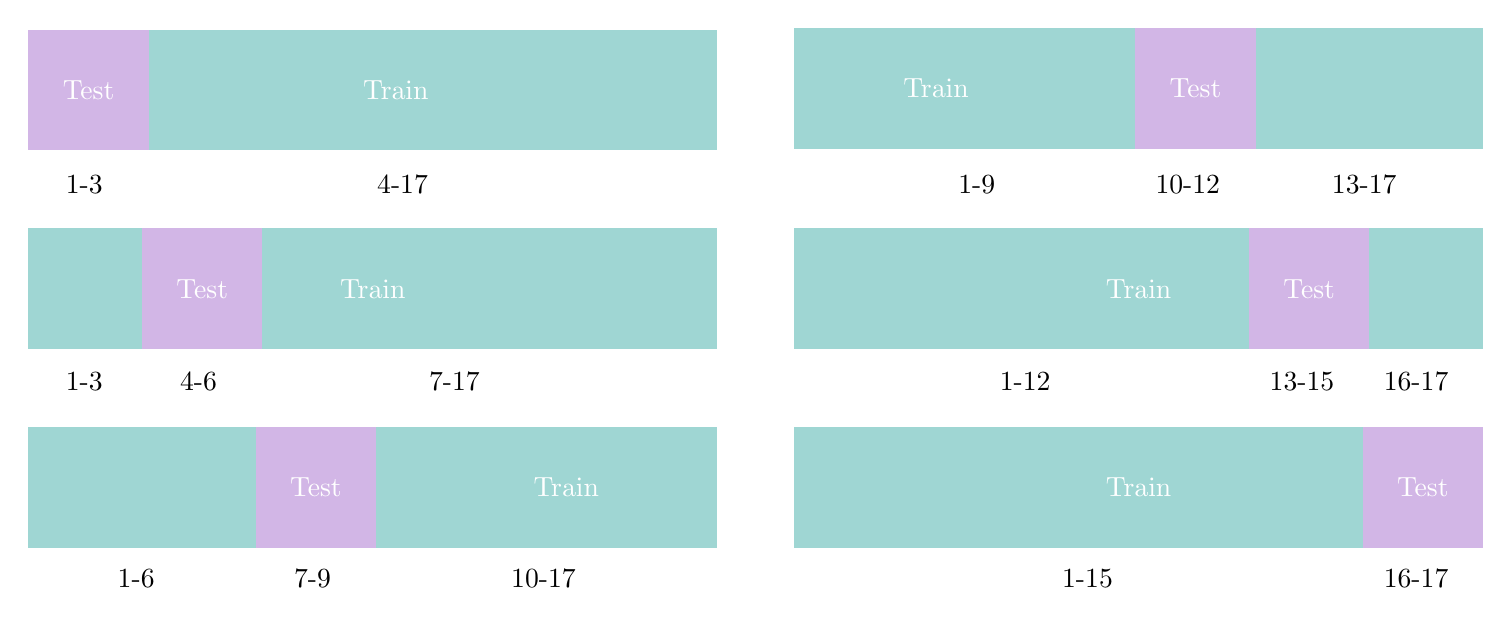
\begin{tikzpicture}[x=0.75pt,y=0.75pt,yscale=-1,xscale=1]
%uncomment if require: \path (0,300); %set diagram left start at 0, and has height of 300


% Text Node
\draw  [draw opacity=0][fill={rgb, 255:red, 159; green, 214; blue, 211 }  ,fill opacity=1 ]  (0.14,-1.35) -- (332.14,-1.35) -- (332.14,56.65) -- (0.14,56.65) -- cycle  ;
\draw (166.14,27.65) node   [align=left] {\begin{minipage}[lt]{223.45pt}\setlength\topsep{0pt}
\begin{center}
\textcolor[rgb]{1,1,1}{ \ \ \ \ \ Train}
\end{center}

\end{minipage}};
% Text Node
\draw  [draw opacity=0][fill={rgb, 255:red, 159; green, 214; blue, 211 }  ,fill opacity=1 ]  (0.14,94.44) -- (332.14,94.44) -- (332.14,152.44) -- (0.14,152.44) -- cycle  ;
\draw (166.14,123.44) node   [align=left] {\begin{minipage}[lt]{223.45pt}\setlength\topsep{0pt}
\begin{center}
\textcolor[rgb]{1,1,1}{Train}
\end{center}

\end{minipage}};
% Text Node
\draw  [draw opacity=0][fill={rgb, 255:red, 210; green, 182; blue, 230 }  ,fill opacity=1 ]  (54.98,94.44) -- (112.98,94.44) -- (112.98,152.44) -- (54.98,152.44) -- cycle  ;
\draw (83.98,123.44) node   [align=left] {\begin{minipage}[lt]{37.24pt}\setlength\topsep{0pt}
\begin{center}
\textcolor[rgb]{1,1,1}{Test}
\end{center}

\end{minipage}};
% Text Node
\draw  [draw opacity=0][fill={rgb, 255:red, 159; green, 214; blue, 211 }  ,fill opacity=1 ]  (0.14,190.23) -- (332.14,190.23) -- (332.14,248.23) -- (0.14,248.23) -- cycle  ;
\draw (166.14,219.23) node   [align=left] {\begin{minipage}[lt]{223.45pt}\setlength\topsep{0pt}
\begin{flushright}
\textcolor[rgb]{1,1,1}{ \ \ \ Train \ \ \ \ \ \ \ \ \ \ \ \ \ \ \ \ \ \ \ \ Train \ \ \ \ \ \ \ \ }
\end{flushright}

\end{minipage}};
% Text Node
\draw  [draw opacity=0][fill={rgb, 255:red, 159; green, 214; blue, 211 }  ,fill opacity=1 ]  (369.14,-2.03) -- (701.14,-2.03) -- (701.14,55.97) -- (369.14,55.97) -- cycle  ;
\draw (535.14,26.97) node   [align=left] {\begin{minipage}[lt]{223.45pt}\setlength\topsep{0pt}
\textcolor[rgb]{1,1,1}{ \ \ \ \ \ \ \ \ Train \ \ \ \ \ \ \ \ \ \ \ \ \ \ \ \ \ \ \ \ Train}
\end{minipage}};
% Text Node
\draw  [draw opacity=0][fill={rgb, 255:red, 159; green, 214; blue, 211 }  ,fill opacity=1 ]  (369.14,94.44) -- (701.14,94.44) -- (701.14,152.44) -- (369.14,152.44) -- cycle  ;
\draw (535.14,123.44) node   [align=left] {\begin{minipage}[lt]{223.45pt}\setlength\topsep{0pt}
\begin{center}
\textcolor[rgb]{1,1,1}{Train}
\end{center}

\end{minipage}};
% Text Node
\draw  [draw opacity=0][fill={rgb, 255:red, 159; green, 214; blue, 211 }  ,fill opacity=1 ]  (369.14,190.23) -- (701.14,190.23) -- (701.14,248.23) -- (369.14,248.23) -- cycle  ;
\draw (535.14,219.23) node   [align=left] {\begin{minipage}[lt]{223.45pt}\setlength\topsep{0pt}
\begin{center}
\textcolor[rgb]{1,1,1}{Train}
\end{center}

\end{minipage}};
% Text Node
\draw  [draw opacity=0][fill={rgb, 255:red, 210; green, 182; blue, 230 }  ,fill opacity=1 ]  (109.75,190.23) -- (167.75,190.23) -- (167.75,248.23) -- (109.75,248.23) -- cycle  ;
\draw (138.75,219.23) node   [align=left] {\begin{minipage}[lt]{37.24pt}\setlength\topsep{0pt}
\begin{center}
\textcolor[rgb]{1,1,1}{Test}
\end{center}

\end{minipage}};
% Text Node
\draw  [draw opacity=0][fill={rgb, 255:red, 210; green, 182; blue, 230 }  ,fill opacity=1 ]  (533.52,-2.03) -- (591.52,-2.03) -- (591.52,55.97) -- (533.52,55.97) -- cycle  ;
\draw (562.52,26.97) node   [align=left] {\begin{minipage}[lt]{37.24pt}\setlength\topsep{0pt}
\begin{center}
\textcolor[rgb]{1,1,1}{Test}
\end{center}

\end{minipage}};
% Text Node
\draw  [draw opacity=0][fill={rgb, 255:red, 210; green, 182; blue, 230 }  ,fill opacity=1 ]  (588.29,94.44) -- (646.29,94.44) -- (646.29,152.44) -- (588.29,152.44) -- cycle  ;
\draw (617.29,123.44) node   [align=left] {\begin{minipage}[lt]{37.24pt}\setlength\topsep{0pt}
\begin{center}
\textcolor[rgb]{1,1,1}{Test}
\end{center}

\end{minipage}};
% Text Node
\draw  [draw opacity=0][fill={rgb, 255:red, 210; green, 182; blue, 230 }  ,fill opacity=1 ]  (643.06,190.23) -- (701.06,190.23) -- (701.06,248.23) -- (643.06,248.23) -- cycle  ;
\draw (672.06,219.23) node   [align=left] {\begin{minipage}[lt]{37.24pt}\setlength\topsep{0pt}
\begin{center}
\textcolor[rgb]{1,1,1}{Test}
\end{center}

\end{minipage}};
% Text Node
\draw (17,67.8) node [anchor=north west][inner sep=0.75pt]  [font=\normalsize] [align=left] {1-3};
% Text Node
\draw (167,67.8) node [anchor=north west][inner sep=0.75pt]  [font=\normalsize] [align=left] {4-17};
% Text Node
\draw (17,162.8) node [anchor=north west][inner sep=0.75pt]  [font=\normalsize] [align=left] {1-3};
% Text Node
\draw (72,162.8) node [anchor=north west][inner sep=0.75pt]  [font=\normalsize] [align=left] {4-6};
% Text Node
\draw (192,162.8) node [anchor=north west][inner sep=0.75pt]  [font=\normalsize] [align=left] {7-17};
% Text Node
\draw (42,257.8) node [anchor=north west][inner sep=0.75pt]  [font=\normalsize] [align=left] {1-6};
% Text Node
\draw (127,257.8) node [anchor=north west][inner sep=0.75pt]  [font=\normalsize] [align=left] {7-9};
% Text Node
\draw (231.59,257.8) node [anchor=north west][inner sep=0.75pt]  [font=\normalsize] [align=left] {10-17};
% Text Node
\draw (446.96,67.8) node [anchor=north west][inner sep=0.75pt]  [font=\normalsize] [align=left] {1-9};
% Text Node
\draw (542,67.8) node [anchor=north west][inner sep=0.75pt]  [font=\normalsize] [align=left] {10-12};
% Text Node
\draw (627,67.8) node [anchor=north west][inner sep=0.75pt]  [font=\normalsize] [align=left] {13-17};
% Text Node
\draw (467,162.8) node [anchor=north west][inner sep=0.75pt]  [font=\normalsize] [align=left] {1-12};
% Text Node
\draw (597,162.8) node [anchor=north west][inner sep=0.75pt]  [font=\normalsize] [align=left] {13-15};
% Text Node
\draw (652,162.8) node [anchor=north west][inner sep=0.75pt]  [font=\normalsize] [align=left] {16-17};
% Text Node
\draw (497,257.8) node [anchor=north west][inner sep=0.75pt]  [font=\normalsize] [align=left] {1-15};
% Text Node
\draw (652,257.8) node [anchor=north west][inner sep=0.75pt]  [font=\normalsize] [align=left] {16-17};
% Text Node
\draw  [draw opacity=0][fill={rgb, 255:red, 210; green, 182; blue, 230 }  ,fill opacity=1 ]  (0.22,-1.35) -- (58.22,-1.35) -- (58.22,56.65) -- (0.22,56.65) -- cycle  ;
\draw (29.22,27.65) node   [align=left] {\begin{minipage}[lt]{37.24pt}\setlength\topsep{0pt}
\begin{center}
\textcolor[rgb]{1,1,1}{Test}
\end{center}

\end{minipage}};


\end{tikzpicture}
            \end{figure}
        Let's start from the first fold:
        \begin{table}[H]
          \centering
          \begin{tabular}{|c|c|c|c|c|c|c|c|c|}
            \hline
            N\textsuperscript{\underline{o}} & System & mount  & price & con & snow & ice & dur & Accegrade \\ \hline
            1 & SK     & F      & 149   & 1.9 & 2.5  & 4.0 & 3.8 & T         \\ \hline
            2 & SRK    & F or R & 520   & 2.1 & 0.8  & 3.8 & 2.3 & F         \\ \hline
            3 & SRK    & F or R & 389   & 2.0 & 2.2  & 3.3 & 4.3 & T         \\ \hline
            \end{tabular}
          \end{table}
        And training set:
        \begin{table}[H]
          \centering
          \begin{tabular}{|c|c|c|c|c|c|c|c|c|}
          \hline
          N\textsuperscript{\underline{o}} & System & mount  & price & con & snow & ice & dur & Accegrade \\ \hline
          4  & SK     & F      & 213   & 1.7 & 2.0  & 2.4 & 3.4 & F         \\ \hline
          5  & SMS    & F or R & 598   & 1.6 & 2.4  & 7   & 2.8 & F         \\ \hline
          6  & SK     & F      & 109   & 2.0 & 1.9  & 2.4 & 3.7 & F         \\ \hline
          7  & SRK    & F or R & 325   & 2.0 & 2.1  & 3.2 & 2.8 & F         \\ \hline
          8  & SMS    & F or R & 498   & 1.5 & 3.3  & 3.5 & 2.0 & T         \\ \hline
          9  & SRK    & F or R & 396   & 2.8 & 2.1  & 3.1 & 2.5 & T         \\ \hline
          10 & SK     & F      & 160   & 1.7 & 1.9  & 1.6 & 3.7 & F         \\ \hline
          11 & SRK    & F or R & 325   & 2.2 & 2.2  & 4.6 & 3.2 & T         \\ \hline
          12 & SRK    & F      & 298   & 2.5 & 2.3  & 3.3 & 2.8 & T         \\ \hline
          13 & SK     & F      & 206   & 1.9 & 1.4  & 1.8 & 2.7 & F         \\ \hline
          14 & SMS    & F or R & 684   & 1.7 & 3.3  & 4.4 & 2.2 & T         \\ \hline
          15 & SK     & F      & 99    & 2.8 & 2.2  & 2.5 & 4.0 & T         \\ \hline
          16 & SK     & F      & 140   & 2.6 & 2.3  & 3.3 & 3.4 & T         \\ \hline
          17 & SK     & F      & 215   & 2.3 & 3.8  & 4.8 & 2.3 & T         \\ \hline
          \end{tabular}
          \end{table}
    For the first example from test set:
    \begin{itemize}
      \item $\text{IntSec} = \langle SK, F, [149, 213], [1.7, 1.9], [2.0, 2.5], [2.4, 4.0], [3.4, 3.8] \rangle$
      \item $\text{Ext} = \langle 4 \rangle \Longrightarrow \text{False}$
    \end{itemize}
    For the second example from test set:
    \begin{itemize}
      \item $\text{IntSec} = \langle *, *, [213, 520], [1.7, 2.1], [0.8, 2.0], [2.4, 3.8], [2.3, 3.4] \rangle$
      \item $\text{Ext} = \langle 4  \rangle \Longrightarrow \text{False}$
    \end{itemize}
    For the third example from test set:
    \begin{itemize}
      \item $\text{IntSec} = \langle *, *, [ 213, 389], [1.7, 2.0], [2.0, 2.2], [2.4, 3.3], [3.4, 4.3] \rangle$
      \item $\text{Ext} = \langle 4 \rangle \Longrightarrow \text{False}$
    \end{itemize}
    Accuracy $33\%$.
    \par
    Second fold:
    \begin{table}[H]
      \centering
      \begin{tabular}{|c|c|c|c|c|c|c|c|c|}
      \hline
      N\textsuperscript{\underline{o}} & System & mount  & price & con & snow & ice & dur & Accegrade \\ \hline
      4 & SK     & F      & 213   & 1.7 & 2.0  & 2.4 & 3.4 & F         \\ \hline
      5 & SMS    & F or R & 598   & 1.6 & 2.4  & 7   & 2.8 & F         \\ \hline
      6 & SK     & F      & 109   & 2.0 & 1.9  & 2.4 & 3.7 & F         \\ \hline
      \end{tabular}
      \end{table}
    Training set:
    \begin{table}[H]
      \centering
      \begin{tabular}{|c|c|c|c|c|c|c|c|c|}
      \hline
      N\textsuperscript{\underline{o}}  & System & mount  & price & con & snow & ice & dur & Accegrade \\ \hline
      1  & SK     & F      & 149   & 1.9 & 2.5  & 4.0 & 3.8 & T         \\ \hline
      2  & SRK    & F or R & 520   & 2.1 & 0.8  & 3.8 & 2.3 & F         \\ \hline
      3  & SRK    & F or R & 389   & 2.0 & 2.2  & 3.3 & 4.3 & T         \\ \hline
      7  & SRK    & F or R & 325   & 2.0 & 2.1  & 3.2 & 2.8 & F        \\ \hline
      8  & SMS    & F or R & 498   & 1.5 & 3.3  & 3.5 & 2.0 & T         \\ \hline
      9  & SRK    & F or R & 396   & 2.8 & 2.1  & 3.1 & 2.5 & T         \\ \hline
      10 & SK     & F      & 160   & 1.7 & 1.9  & 1.6 & 3.7 & F         \\ \hline
      11 & SRK    & F or R & 325   & 2.2 & 2.2  & 4.6 & 3.2 & T         \\ \hline
      12 & SRK    & F      & 298   & 2.5 & 2.3  & 3.3 & 2.8 & T         \\ \hline
      13 & SK     & F      & 206   & 1.9 & 1.4  & 1.8 & 2.7 & F         \\ \hline
      14 & SMS    & F or R & 684   & 1.7 & 3.3  & 4.4 & 2.2 & T         \\ \hline
      15 & SK     & F      & 99    & 2.8 & 2.2  & 2.5 & 4.0 & T         \\ \hline
      16 & SK     & F      & 140   & 2.6 & 2.3  & 3.3 & 3.4 & T         \\ \hline
      17 & SK     & F      & 215   & 2.3 & 3.8  & 4.8 & 2.3 & T         \\ \hline
      \end{tabular}
      \end{table}
      The first test example:
      \begin{itemize}
        \item $\text{IntSec} = \langle SK, F, [ 149, 213], [1.7, 1.9], [2.0, 2.5], [2.4, 4.0], [3.4, 3.8] \rangle$
        \item $\text{Ext} = \langle 1 \rangle \Longrightarrow \text{True}$
      \end{itemize}
      The second test example:
      \begin{itemize}
        \item $\text{IntSec} = \langle *, *, [ 149, 598], [1.6, 1.9], [2.4, 2.5], [4.0, 7], [2.8, 3.8] \rangle$
        \item $\text{Ext} = \langle 1 \rangle \Longrightarrow \text{True}$
      \end{itemize}
      The third test example:
      \begin{itemize}
        \item $\text{IntSec} = \langle SK, F, [ 109, 149], [1.9, 2.0], [1.9, 2.5], [2.4, 4.0], [3.7, 3.8] \rangle$
        \item $\text{Ext} = \langle 1 \rangle \Longrightarrow \text{True}$
      \end{itemize}
      Accuracy: $0\%$.
      \par 
      Third fold:
      \begin{table}[H]
        \centering
        \begin{tabular}{|c|c|c|c|c|c|c|c|c|}
        \hline
        N\textsuperscript{\underline{o}} & System & mount  & price & con & snow & ice & dur & Accegrade \\ \hline
        7 & SRK    & F or R & 325   & 2.0 & 2.1  & 3.2 & 2.8 & F         \\ \hline
        8 & SMS    & F or R & 498   & 1.5 & 3.3  & 3.5 & 2.0 & T         \\ \hline
        9 & SRK    & F or R & 396   & 2.8 & 2.1  & 3.1 & 2.5 & T         \\ \hline
        \end{tabular}
        \end{table}
        Train set:
        \begin{table}[H]
          \centering
          \begin{tabular}{|c|c|c|c|c|c|c|c|c|}
          \hline
          N\textsuperscript{\underline{o}}  & System & mount  & price & con & snow & ice & dur & Accegrade \\ \hline
          1  & SK     & F      & 149   & 1.9 & 2.5  & 4.0 & 3.8 & T         \\ \hline
          2  & SRK    & F or R & 520   & 2.1 & 0.8  & 3.8 & 2.3 & F         \\ \hline
          3  & SRK    & F or R & 389   & 2.0 & 2.2  & 3.3 & 4.3 & T         \\ \hline
          4  & SK     & F      & 213   & 1.7 & 2.0  & 2.4 & 3.4 & F         \\ \hline
          5  & SMS    & F or R & 598   & 1.6 & 2.4  & 7   & 2.8 & F         \\ \hline
          6  & SK     & F      & 109   & 2.0 & 1.9  & 2.4 & 3.7 & F         \\ \hline
          10 & SK     & F      & 160   & 1.7 & 1.9  & 1.6 & 3.7 & F         \\ \hline
          11 & SRK    & F or R & 325   & 2.2 & 2.2  & 4.6 & 3.2 & T         \\ \hline
          12 & SRK    & F      & 298   & 2.5 & 2.3  & 3.3 & 2.8 & T         \\ \hline
          13 & SK     & F      & 206   & 1.9 & 1.4  & 1.8 & 2.7 & F         \\ \hline
          14 & SMS    & F or R & 684   & 1.7 & 3.3  & 4.4 & 2.2 & T         \\ \hline
          15 & SK     & F      & 99    & 2.8 & 2.2  & 2.5 & 4.0 & T         \\ \hline
          16 & SK     & F      & 140   & 2.6 & 2.3  & 3.3 & 3.4 & T         \\ \hline
          17 & SK     & F      & 215   & 2.3 & 3.8  & 4.8 & 2.3 & T         \\ \hline
          \end{tabular}
          \end{table}
      The first test example:
      \begin{itemize}
        \item $\text{IntSec} = \langle *, *, [ 149, 325], [1.9, 2.0], [2.1, 2.5], [3.2, 4.0], [2.8, 3.8] \rangle$
        \item $\text{Ext} = \langle 1 \rangle \Longrightarrow \text{True}$
      \end{itemize}
      The second test example:
      \begin{itemize}
        \item $\text{IntSec} = \langle *, *, [ 149, 498], [1.5, 1.9], [2.5, 3.3], [3.5, 4.0], [2.0, 3.8] \rangle$
        \item $\text{Ext} = \langle 1 \rangle \Longrightarrow \text{True}$
      \end{itemize}
      The third test example:
      \begin{itemize}
        \item $\text{IntSec} = \langle *, *, [ 149, 396], [1.9, 2.8], [2.1, 2.5], [3.1, 4.0], [2.5, 3.8] \rangle$
        \item $\text{Ext} = \langle 1, 12 \rangle \Longrightarrow \text{True}$
      \end{itemize}
      Accuracy: $67\%$.
      \par 
      Fourth fold:
      \begin{table}[H]
        \centering
        \begin{tabular}{|c|c|c|c|c|c|c|c|c|}
        \hline
        N\textsuperscript{\underline{o}} & System & mount  & price & con & snow & ice & dur & Accegrade \\ \hline
        10 & SK     & F      & 160   & 1.7 & 1.9  & 1.6 & 3.7 & F         \\ \hline
        11 & SRK    & F or R & 325   & 2.2 & 2.2  & 4.6 & 3.2 & T         \\ \hline
        12 & SRK    & F      & 298   & 2.5 & 2.3  & 3.3 & 2.8 & T         \\ \hline
        \end{tabular}
        \end{table}
      Train set:
      \begin{table}[H]
        \centering
        \begin{tabular}{|c|c|c|c|c|c|c|c|c|}
        \hline
        N\textsuperscript{\underline{o}} & System & mount  & price & con & snow & ice & dur & Accegrade \\ \hline
        1  & SK     & F      & 149   & 1.9 & 2.5  & 4.0 & 3.8 & T         \\ \hline
        2  & SRK    & F or R & 520   & 2.1 & 0.8  & 3.8 & 2.3 & F         \\ \hline
        3  & SRK    & F or R & 389   & 2.0 & 2.2  & 3.3 & 4.3 & T         \\ \hline
        4  & SK     & F      & 213   & 1.7 & 2.0  & 2.4 & 3.4 & F         \\ \hline
        5  & SMS    & F or R & 598   & 1.6 & 2.4  & 7   & 2.8 & F         \\ \hline
        6  & SK     & F      & 109   & 2.0 & 1.9  & 2.4 & 3.7 & F         \\ \hline
        7  & SRK    & F or R & 325   & 2.0 & 2.1  & 3.2 & 2.8 & F         \\ \hline
        8  & SMS    & F or R & 498   & 1.5 & 3.3  & 3.5 & 2.0 & T         \\ \hline
        9  & SRK    & F or R & 396   & 2.8 & 2.1  & 3.1 & 2.5 & T         \\ \hline
        13 & SK     & F      & 206   & 1.9 & 1.4  & 1.8 & 2.7 & F         \\ \hline
        14 & SMS    & F or R & 684   & 1.7 & 3.3  & 4.4 & 2.2 & T         \\ \hline
        15 & SK     & F      & 99    & 2.8 & 2.2  & 2.5 & 4.0 & T         \\ \hline
        16 & SK     & F      & 140   & 2.6 & 2.3  & 3.3 & 3.4 & T         \\ \hline
        17 & SK     & F      & 215   & 2.3 & 3.8  & 4.8 & 2.3 & T         \\ \hline
        \end{tabular}
        \end{table}
      The first test example:
      \begin{itemize}
        \item $\text{IntSec} = \langle SK, F, [ 149, 160], [1.7, 1.9], [1.9, 2.5], [1.6, 4.0], [3.7, 3.8] \rangle$
        \item $\text{Ext} = \langle 1 \rangle \Longrightarrow \text{True}$
      \end{itemize}
      The second test example:
      \begin{itemize}
        \item $\text{IntSec} = \langle *, *, [ 149, 325], [1.9, 2.2], [2.2, 2.5], [4.0, 4.6], [3.2, 3.8] \rangle$
        \item $\text{Ext} = \langle 1 \rangle \Longrightarrow \text{True}$
      \end{itemize}
      The third test example:
      \begin{itemize}
        \item $\text{IntSec} = \langle *, F, [ 149, 298], [1.9, 2.5], [2.3, 2.5], [3.3, 4.0], [2.8, 3.8] \rangle$
        \item $\text{Ext} = \langle 1 \rangle \Longrightarrow \text{True}$
      \end{itemize}
      Accuracy: $67\%$.
      \par 
      Fifth fold:
      \begin{table}[H]
        \centering
        \begin{tabular}{|c|c|c|c|c|c|c|c|c|}
        \hline
        N\textsuperscript{\underline{o}} & System & mount  & price & con & snow & ice & dur & Accegrade \\ \hline
        13 & SK     & F      & 206   & 1.9 & 1.4  & 1.8 & 2.7 & F         \\ \hline
        14 & SMS    & F or R & 684   & 1.7 & 3.3  & 4.4 & 2.2 & T         \\ \hline
        15 & SK     & F      & 99    & 2.8 & 2.2  & 2.5 & 4.0 & T         \\ \hline
        \end{tabular}
        \end{table}
    Train set is presented in Table \ref{table:cv_train}:
    \par 
    The first test example:
    \begin{itemize}
      \item $\text{IntSec} = \langle SK, F, [ 149, 206], [1.9, 1.9], [1.4, 2.5], [1.8, 4.0], [2.7, 3.8] \rangle$
      \item $\text{Ext} = \langle 1 \rangle \Longrightarrow \text{True}$
    \end{itemize}
    \begin{table}[H]
      \centering
      \begin{tabular}{|c|c|c|c|c|c|c|c|c|}
      \hline
      N\textsuperscript{\underline{o}} & System & mount  & price & con & snow & ice & dur & Accegrade \\ \hline
      1  & SK     & F      & 149   & 1.9 & 2.5  & 4.0 & 3.8 & T         \\ \hline
      2  & SRK    & F or R & 520   & 2.1 & 0.8  & 3.8 & 2.3 & F         \\ \hline
      3  & SRK    & F or R & 389   & 2.0 & 2.2  & 3.3 & 4.3 & T         \\ \hline
      4  & SK     & F      & 213   & 1.7 & 2.0  & 2.4 & 3.4 & F         \\ \hline
      5  & SMS    & F or R & 598   & 1.6 & 2.4  & 7   & 2.8 & F         \\ \hline
      6  & SK     & F      & 109   & 2.0 & 1.9  & 2.4 & 3.7 & F         \\ \hline
      7  & SRK    & F or R & 325   & 2.0 & 2.1  & 3.2 & 2.8 & F         \\ \hline
      8  & SMS    & F or R & 498   & 1.5 & 3.3  & 3.5 & 2.0 & T         \\ \hline
      9  & SRK    & F or R & 396   & 2.8 & 2.1  & 3.1 & 2.5 & T         \\ \hline
      10 & SK     & F      & 160   & 1.7 & 1.9  & 1.6 & 3.7 & F         \\ \hline
      11 & SRK    & F or R & 325   & 2.2 & 2.2  & 4.6 & 3.2 & T         \\ \hline
      12 & SRK    & F      & 298   & 2.5 & 2.3  & 3.3 & 2.8 & T         \\ \hline
      16 & SK     & F      & 140   & 2.6 & 2.3  & 3.3 & 3.4 & T         \\ \hline
      17 & SK     & F      & 215   & 2.3 & 3.8  & 4.8 & 2.3 & T         \\ \hline
      \end{tabular}
      \caption{CV train set for fifth fold}
      \label{table:cv_train}
      \end{table}
    The second test example:
    \begin{itemize}
      \item $\text{IntSec} = \langle *, *, [ 149, 684], [1.7, 1.9], [2.5, 3.3], [4.0, 4.4], [2.2, 3.8] \rangle$
      \item $\text{Ext} = \langle 1 \rangle \Longrightarrow \text{True}$
    \end{itemize}
    The third test example:
    \begin{itemize}
      \item $\text{IntSec} = \langle SK, F, [ 99, 149], [1.9, 2.8], [2.2, 2.5], [2.5, 4.0], [3.8, 4.0] \rangle$
      \item $\text{Ext} = \langle 1 \rangle \Longrightarrow \text{True}$
    \end{itemize}
    Accuracy: $67\%$.
    \par 
    Last fold:
    \begin{table}[H]
      \centering
      \begin{tabular}{|c|c|c|c|c|c|c|c|c|}
      \hline
      N\textsuperscript{\underline{o}} & System & mount & price & con & snow & ice & dur & Accegrade \\ \hline
      16 & SK     & F     & 140   & 2.6 & 2.3  & 3.3 & 3.4 & T         \\ \hline
      17 & SK     & F     & 215   & 2.3 & 3.8  & 4.8 & 2.3 & T         \\ \hline
      \end{tabular}
      \end{table}
      Train set is presented in Table \ref{table:cv_train2}
      \par
      The first test example:
      \begin{itemize}
        \item $\text{IntSec} = \langle SK, F, [ 140, 149], [1.9, 2.6], [2.3, 2.5], [3.3, 4.0], [3.4, 3.8] \rangle$
        \item $\text{Ext} = \langle 1 \rangle \Longrightarrow \text{True}$
      \end{itemize}
      The second test example:
      \begin{itemize}
        \item $\text{IntSec} = \langle SK, F, [ 149, 215], [1.9, 2.3], [2.5, 3.8], [4.0, 4.8], [2.3, 3.8] \rangle$
        \item $\text{Ext} = \langle 1 \rangle \Longrightarrow \text{True}$
      \end{itemize}
      \begin{table}[H]
        \centering
        \begin{tabular}{|c|c|c|c|c|c|c|c|c|}
        \hline
        N\textsuperscript{\underline{o}} & System & mount  & price & con & snow & ice & dur & Accegrade \\ \hline
        1  & SK     & F      & 149   & 1.9 & 2.5  & 4.0 & 3.8 & T         \\ \hline
        2  & SRK    & F or R & 520   & 2.1 & 0.8  & 3.8 & 2.3 & F         \\ \hline
        3  & SRK    & F or R & 389   & 2.0 & 2.2  & 3.3 & 4.3 & T         \\ \hline
        4  & SK     & F      & 213   & 1.7 & 2.0  & 2.4 & 3.4 & F         \\ \hline
        5  & SMS    & F or R & 598   & 1.6 & 2.4  & 7   & 2.8 & F         \\ \hline
        6  & SK     & F      & 109   & 2.0 & 1.9  & 2.4 & 3.7 & F         \\ \hline
        7  & SRK    & F or R & 325   & 2.0 & 2.1  & 3.2 & 2.8 & F         \\ \hline
        8  & SMS    & F or R & 498   & 1.5 & 3.3  & 3.5 & 2.0 & T         \\ \hline
        9  & SRK    & F or R & 396   & 2.8 & 2.1  & 3.1 & 2.5 & T         \\ \hline
        10 & SK     & F      & 160   & 1.7 & 1.9  & 1.6 & 3.7 & F         \\ \hline
        11 & SRK    & F or R & 325   & 2.2 & 2.2  & 4.6 & 3.2 & T         \\ \hline
        12 & SRK    & F      & 298   & 2.5 & 2.3  & 3.3 & 2.8 & T         \\ \hline
        13 & SK     & F      & 206   & 1.9 & 1.4  & 1.8 & 2.7 & F         \\ \hline
        14 & SMS    & F or R & 684   & 1.7 & 3.3  & 4.4 & 2.2 & T         \\ \hline
        15 & SK     & F      & 99    & 2.8 & 2.2  & 2.5 & 4.0 & T         \\ \hline
        \end{tabular}
        \caption{CV train set for sixth fold}
        \label{table:cv_train2}
        \end{table}
      Accuracy: $100\%$.
      \par 
      Accuracy through cross-validation: $55.67\%$.
      \item New definition of intersection on interval patterns:
      \[
        [a_1, \infty] \cap [a_2, \infty] = [\min (a_1, a_2), \infty].
      \]
      Let's classify the fifteenth object. Train set
      \begin{table}[H]
        \centering
          \begin{tabular}{|c|c|c|c|c|c|c|c|c|}
          \hline
          N\textsuperscript{\underline{o}} & System & mount  & price & con & snow & ice & dur & Accegrade \\ \hline
          1  & SK     & F      & 149   & 1.9 & 2.5  & 4.0 & 3.8 & T         \\ \hline
          2  & SRK    & F or R & 520   & 2.1 & 0.8  & 3.8 & 2.3 & F         \\ \hline
          3  & SRK    & F or R & 389   & 2.0 & 2.2  & 3.3 & 4.3 & T         \\ \hline
          4  & SK     & F      & 213   & 1.7 & 2.0  & 2.4 & 3.4 & F         \\ \hline
          5  & SMS    & F or R & 598   & 1.6 & 2.4  & 7   & 2.8 & F         \\ \hline
          6  & SK     & F      & 109   & 2.0 & 1.9  & 2.4 & 3.7 & F         \\ \hline
          7  & SRK    & F or R & 325   & 2.0 & 2.1  & 3.2 & 2.8 & F         \\ \hline
          8  & SMS    & F or R & 498   & 1.5 & 3.3  & 3.5 & 2.0 & T         \\ \hline
          9  & SRK    & F or R & 396   & 2.8 & 2.1  & 3.1 & 2.5 & T         \\ \hline
          10 & SK     & F      & 160   & 1.7 & 1.9  & 1.6 & 3.7 & F         \\ \hline
          11 & SRK    & F or R & 325   & 2.2 & 2.2  & 4.6 & 3.2 & T         \\ \hline
          12 & SRK    & F      & 298   & 2.5 & 2.3  & 3.3 & 2.8 & T         \\ \hline
          13 & SK     & F      & 206   & 1.9 & 1.4  & 1.8 & 2.7 & F         \\ \hline
          14 & SMS    & F or R & 684   & 1.7 & 3.3  & 4.4 & 2.2 & T         \\ \hline
          16 & SK     & F      & 140   & 2.6 & 2.3  & 3.3 & 3.4 & T         \\ \hline
          17 & SK     & F      & 215   & 2.3 & 3.8  & 4.8 & 2.3 & T         \\ \hline
          \end{tabular}
          \end{table}

          \begin{table}[H]
            \centering
            \begin{tabular}{|c|c|c|c|c|c|c|c|c|}
            \hline
            N\textsuperscript{\underline{o}} & System & mount & price & con & snow & ice & dur & Accegrade \\ \hline
            15 & SK     & F     & 99    & 2.8 & 2.2  & 2.5 & 4.0 & T         \\ \hline
            \end{tabular}
            \end{table}
            \begin{itemize}
              \item $\text{IntSec} = \langle SK, F, [ 99, \infty], [1.9, \infty], [2.2, \infty], [2.5, \infty], [3.8, \infty] \rangle$
              \item $\text{Ext} = \langle 1 \rangle \Longrightarrow \text{True}$
            \end{itemize} 
        \item Another definition of intersection on interval patterns:
        \[[a_1, \infty] \cap [a_2, \infty] = [\max (a_1, a_2), \infty].\]
        \begin{itemize}
          \item $\text{IntSec} = \langle SK, F, [ 149, \infty], [2.8, \infty], [2.5, \infty], [4.0, \infty], [4.0, \infty] \rangle$
          \item $\text{Ext} = \langle 1 \rangle \Longrightarrow \text{True}$
        \end{itemize}
        The definition from the 4th subtask is more suitable for our dataset. In general, if the test example will have the maximum element, then we will obtain undefined extension.
    \end{enumerate}
\end{solution}

\begin{problem}{}
    Given the molecular graphs of 4 example substances belonging to the positive class and 3 example substances belonging to the negative class. Using the JSM method, construct pattern concept lattices for the positive (objects $G_1, \ldots, G_4$) and negative (objects $G_5, \ldots, G_7$) contexts, find their respective minimum positive and negative hypotheses and classify the test examples (objects $G_8, \ldots, G_{11}$), accordingly.
    
    \subsection*{Positive examples}
    \begin{figure}[H]
        \centering

\tikzset{every picture/.style={line width=0.75pt}} %set default line width to 0.75pt        

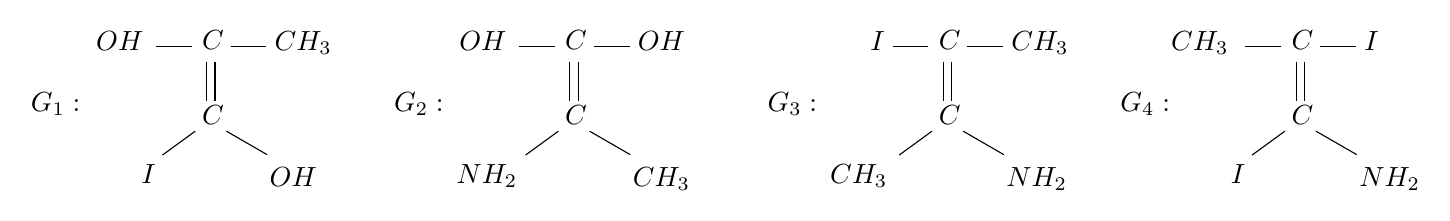
\begin{tikzpicture}[x=0.75pt,y=0.75pt,yscale=-1,xscale=1]
%uncomment if require: \path (0,300); %set diagram left start at 0, and has height of 300

%Straight Lines [id:da846897062150809] 
\draw    (73,50.9) -- (90.29,50.9) ;
%Straight Lines [id:da5233570107936059] 
\draw    (109,50.9) -- (126.29,50.9) ;
%Straight Lines [id:da3570392511339686] 
\draw    (97.5,58.4) -- (97.5,77.4) ;
%Straight Lines [id:da5668461539599012] 
\draw    (101.5,58.4) -- (101.5,77.4) ;
%Straight Lines [id:da9335814717191053] 
\draw    (92,91.9) -- (76.2,103.41) ;
%Straight Lines [id:da4145258485980037] 
\draw    (126.61,103.2) -- (107,91.9) ;
%Straight Lines [id:da7798712844995945] 
\draw    (247.97,50.9) -- (265.26,50.9) ;
%Straight Lines [id:da6973389335797833] 
\draw    (283.97,50.9) -- (301.26,50.9) ;
%Straight Lines [id:da9972403694018135] 
\draw    (272.47,58.4) -- (272.47,77.4) ;
%Straight Lines [id:da23702841316511147] 
\draw    (276.47,58.4) -- (276.47,77.4) ;
%Straight Lines [id:da9764825376266975] 
\draw    (266.97,91.9) -- (251.17,103.41) ;
%Straight Lines [id:da8564770361796279] 
\draw    (301.57,103.2) -- (281.97,91.9) ;
%Straight Lines [id:da5805176197697994] 
\draw    (427.97,50.9) -- (445.26,50.9) ;
%Straight Lines [id:da25047126237464146] 
\draw    (463.97,50.9) -- (481.26,50.9) ;
%Straight Lines [id:da25124366061166703] 
\draw    (452.47,58.4) -- (452.47,77.4) ;
%Straight Lines [id:da894769536915182] 
\draw    (456.47,58.4) -- (456.47,77.4) ;
%Straight Lines [id:da5110832636857212] 
\draw    (446.97,91.9) -- (431.17,103.41) ;
%Straight Lines [id:da5912747311016606] 
\draw    (481.57,103.2) -- (461.97,91.9) ;
%Straight Lines [id:da3148852790405936] 
\draw    (597.97,50.9) -- (615.26,50.9) ;
%Straight Lines [id:da3387786073545902] 
\draw    (633.97,50.9) -- (651.26,50.9) ;
%Straight Lines [id:da07829059016645101] 
\draw    (622.47,58.4) -- (622.47,77.4) ;
%Straight Lines [id:da3415347439551548] 
\draw    (626.47,58.4) -- (626.47,77.4) ;
%Straight Lines [id:da6369740816090996] 
\draw    (616.97,91.9) -- (601.17,103.41) ;
%Straight Lines [id:da342082099953833] 
\draw    (651.57,103.2) -- (631.97,91.9) ;

% Text Node
\draw (11.53,71.97) node [anchor=north west][inner sep=0.75pt]   [align=left] {$\displaystyle G_{1} :$};
% Text Node
\draw (43,42.7) node [anchor=north west][inner sep=0.75pt]   [align=left] {$\displaystyle OH$};
% Text Node
\draw (129,42.7) node [anchor=north west][inner sep=0.75pt]   [align=left] {$\displaystyle CH_{3}$};
% Text Node
\draw (94,42.3) node [anchor=north west][inner sep=0.75pt]   [align=left] {$\displaystyle C$};
% Text Node
\draw (64.73,106.77) node [anchor=north west][inner sep=0.75pt]   [align=left] {$\displaystyle I$};
% Text Node
\draw (94,78.38) node [anchor=north west][inner sep=0.75pt]   [align=left] {$\displaystyle C$};
% Text Node
\draw (126.61,108) node [anchor=north west][inner sep=0.75pt]   [align=left] {$\displaystyle OH$};
% Text Node
\draw (186.5,71.97) node [anchor=north west][inner sep=0.75pt]   [align=left] {$\displaystyle G_{2} :$};
% Text Node
\draw (217.97,42.7) node [anchor=north west][inner sep=0.75pt]   [align=left] {$\displaystyle OH$};
% Text Node
\draw (303.97,42.7) node [anchor=north west][inner sep=0.75pt]   [align=left] {$\displaystyle OH$};
% Text Node
\draw (268.97,42.3) node [anchor=north west][inner sep=0.75pt]   [align=left] {$\displaystyle C$};
% Text Node
\draw (216.67,106.77) node [anchor=north west][inner sep=0.75pt]   [align=left] {$\displaystyle NH_{2}$};
% Text Node
\draw (268.97,78.38) node [anchor=north west][inner sep=0.75pt]   [align=left] {$\displaystyle C$};
% Text Node
\draw (301.57,108) node [anchor=north west][inner sep=0.75pt]   [align=left] {$\displaystyle CH_{3}$};
% Text Node
\draw (366.5,71.97) node [anchor=north west][inner sep=0.75pt]   [align=left] {$\displaystyle G_{3} :$};
% Text Node
\draw (415.97,42.8) node [anchor=north west][inner sep=0.75pt]   [align=left] {$\displaystyle I$};
% Text Node
\draw (483.97,42.7) node [anchor=north west][inner sep=0.75pt]   [align=left] {$\displaystyle CH_{3}$};
% Text Node
\draw (448.97,42.3) node [anchor=north west][inner sep=0.75pt]   [align=left] {$\displaystyle C$};
% Text Node
\draw (396.67,106.77) node [anchor=north west][inner sep=0.75pt]   [align=left] {$\displaystyle CH_{3}$};
% Text Node
\draw (448.97,78.38) node [anchor=north west][inner sep=0.75pt]   [align=left] {$\displaystyle C$};
% Text Node
\draw (481.57,108) node [anchor=north west][inner sep=0.75pt]   [align=left] {$\displaystyle NH_{2}$};
% Text Node
\draw (536.5,71.97) node [anchor=north west][inner sep=0.75pt]   [align=left] {$\displaystyle G_{4} :$};
% Text Node
\draw (560.97,42.7) node [anchor=north west][inner sep=0.75pt]   [align=left] {$\displaystyle CH_{3}$};
% Text Node
\draw (653.97,42.7) node [anchor=north west][inner sep=0.75pt]   [align=left] {$\displaystyle I$};
% Text Node
\draw (618.97,42.3) node [anchor=north west][inner sep=0.75pt]   [align=left] {$\displaystyle C$};
% Text Node
\draw (589.7,106.77) node [anchor=north west][inner sep=0.75pt]   [align=left] {$\displaystyle I$};
% Text Node
\draw (618.97,78.38) node [anchor=north west][inner sep=0.75pt]   [align=left] {$\displaystyle C$};
% Text Node
\draw (651.57,108) node [anchor=north west][inner sep=0.75pt]   [align=left] {$\displaystyle NH_{2}$};
\end{tikzpicture}
    \end{figure}

    \subsection*{Negative examples}

    \begin{figure}[H]
        \centering
        

\tikzset{every picture/.style={line width=0.75pt}} %set default line width to 0.75pt        

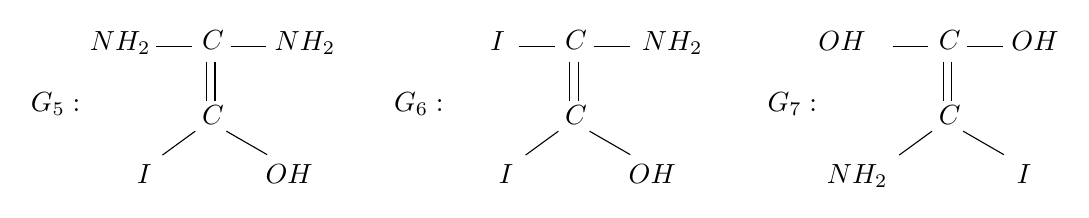
\begin{tikzpicture}[x=0.75pt,y=0.75pt,yscale=-1,xscale=1]
%uncomment if require: \path (0,300); %set diagram left start at 0, and has height of 300

%Straight Lines [id:da958741346337896] 
\draw    (63,70.9) -- (80.29,70.9) ;
%Straight Lines [id:da43463851458081426] 
\draw    (99,70.9) -- (116.29,70.9) ;
%Straight Lines [id:da020193889328386838] 
\draw    (87.5,78.4) -- (87.5,97.4) ;
%Straight Lines [id:da4354281449179227] 
\draw    (91.5,78.4) -- (91.5,97.4) ;
%Straight Lines [id:da4196312433333844] 
\draw    (82,111.9) -- (66.2,123.41) ;
%Straight Lines [id:da2827011702098936] 
\draw    (116.61,123.2) -- (97,111.9) ;
%Straight Lines [id:da3754668548597775] 
\draw    (237.97,70.9) -- (255.26,70.9) ;
%Straight Lines [id:da9709319848614761] 
\draw    (273.97,70.9) -- (291.26,70.9) ;
%Straight Lines [id:da9856442682267186] 
\draw    (262.47,78.4) -- (262.47,97.4) ;
%Straight Lines [id:da28105285911948186] 
\draw    (266.47,78.4) -- (266.47,97.4) ;
%Straight Lines [id:da8973563155618876] 
\draw    (256.97,111.9) -- (241.17,123.41) ;
%Straight Lines [id:da9781003408982767] 
\draw    (291.57,123.2) -- (271.97,111.9) ;
%Straight Lines [id:da6567368170981687] 
\draw    (417.97,70.9) -- (435.26,70.9) ;
%Straight Lines [id:da8511145764962567] 
\draw    (453.97,70.9) -- (471.26,70.9) ;
%Straight Lines [id:da7522910467439474] 
\draw    (442.47,78.4) -- (442.47,97.4) ;
%Straight Lines [id:da7763411848769071] 
\draw    (446.47,78.4) -- (446.47,97.4) ;
%Straight Lines [id:da07684339094782766] 
\draw    (436.97,111.9) -- (421.17,123.41) ;
%Straight Lines [id:da11734471241731037] 
\draw    (471.57,123.2) -- (451.97,111.9) ;

% Text Node
\draw (1.53,91.97) node [anchor=north west][inner sep=0.75pt]   [align=left] {$\displaystyle G_{5} :$};
% Text Node
\draw (30,62.7) node [anchor=north west][inner sep=0.75pt]   [align=left] {$\displaystyle NH_{2}$};
% Text Node
\draw (119,62.7) node [anchor=north west][inner sep=0.75pt]   [align=left] {$\displaystyle NH_{2}$};
% Text Node
\draw (84,62.3) node [anchor=north west][inner sep=0.75pt]   [align=left] {$\displaystyle C$};
% Text Node
\draw (52.73,126.77) node [anchor=north west][inner sep=0.75pt]   [align=left] {$\displaystyle I$};
% Text Node
\draw (84,98.38) node [anchor=north west][inner sep=0.75pt]   [align=left] {$\displaystyle C$};
% Text Node
\draw (114.61,126.8) node [anchor=north west][inner sep=0.75pt]   [align=left] {$\displaystyle OH$};
% Text Node
\draw (176.5,91.97) node [anchor=north west][inner sep=0.75pt]   [align=left] {$\displaystyle G_{6} :$};
% Text Node
\draw (222.97,62.7) node [anchor=north west][inner sep=0.75pt]   [align=left] {$\displaystyle I$};
% Text Node
\draw (295.97,62.7) node [anchor=north west][inner sep=0.75pt]   [align=left] {$\displaystyle NH_{2}$};
% Text Node
\draw (258.97,62.3) node [anchor=north west][inner sep=0.75pt]   [align=left] {$\displaystyle C$};
% Text Node
\draw (227,126.77) node [anchor=north west][inner sep=0.75pt]   [align=left] {$\displaystyle I$};
% Text Node
\draw (258.97,98.38) node [anchor=north west][inner sep=0.75pt]   [align=left] {$\displaystyle C$};
% Text Node
\draw (289.57,126.8) node [anchor=north west][inner sep=0.75pt]   [align=left] {$\displaystyle OH$};
% Text Node
\draw (356.5,91.97) node [anchor=north west][inner sep=0.75pt]   [align=left] {$\displaystyle G_{7} :$};
% Text Node
\draw (380.97,62.8) node [anchor=north west][inner sep=0.75pt]   [align=left] {$\displaystyle OH$};
% Text Node
\draw (473.97,62.7) node [anchor=north west][inner sep=0.75pt]   [align=left] {$\displaystyle OH$};
% Text Node
\draw (438.97,62.3) node [anchor=north west][inner sep=0.75pt]   [align=left] {$\displaystyle C$};
% Text Node
\draw (385,126.77) node [anchor=north west][inner sep=0.75pt]   [align=left] {$\displaystyle NH_{2}$};
% Text Node
\draw (438.97,98.38) node [anchor=north west][inner sep=0.75pt]   [align=left] {$\displaystyle C$};
% Text Node
\draw (476.57,126.8) node [anchor=north west][inner sep=0.75pt]   [align=left] {$\displaystyle I$};


\end{tikzpicture}
    \end{figure}

    \subsection*{Test examples}
    \begin{figure}[H]
        \centering
        

\tikzset{every picture/.style={line width=0.75pt}} %set default line width to 0.75pt        

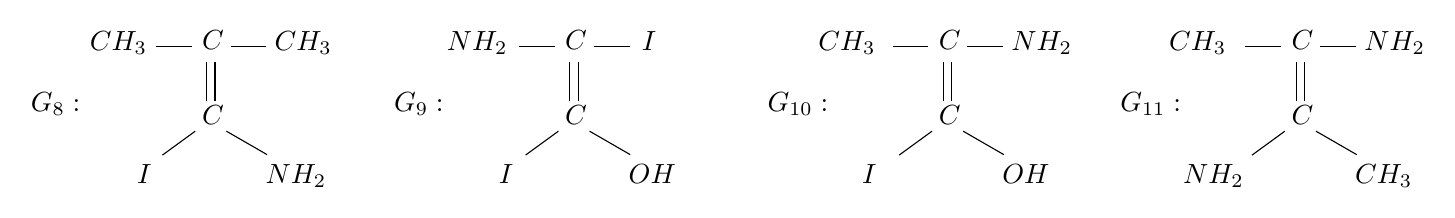
\begin{tikzpicture}[x=0.75pt,y=0.75pt,yscale=-1,xscale=1]
%uncomment if require: \path (0,300); %set diagram left start at 0, and has height of 300

%Straight Lines [id:da846897062150809] 
\draw    (73,50.9) -- (90.29,50.9) ;
%Straight Lines [id:da5233570107936059] 
\draw    (109,50.9) -- (126.29,50.9) ;
%Straight Lines [id:da3570392511339686] 
\draw    (97.5,58.4) -- (97.5,77.4) ;
%Straight Lines [id:da5668461539599012] 
\draw    (101.5,58.4) -- (101.5,77.4) ;
%Straight Lines [id:da9335814717191053] 
\draw    (92,91.9) -- (76.2,103.41) ;
%Straight Lines [id:da4145258485980037] 
\draw    (126.61,103.2) -- (107,91.9) ;
%Straight Lines [id:da7798712844995945] 
\draw    (247.97,50.9) -- (265.26,50.9) ;
%Straight Lines [id:da6973389335797833] 
\draw    (283.97,50.9) -- (301.26,50.9) ;
%Straight Lines [id:da9972403694018135] 
\draw    (272.47,58.4) -- (272.47,77.4) ;
%Straight Lines [id:da23702841316511147] 
\draw    (276.47,58.4) -- (276.47,77.4) ;
%Straight Lines [id:da9764825376266975] 
\draw    (266.97,91.9) -- (251.17,103.41) ;
%Straight Lines [id:da8564770361796279] 
\draw    (301.57,103.2) -- (281.97,91.9) ;
%Straight Lines [id:da5805176197697994] 
\draw    (427.97,50.9) -- (445.26,50.9) ;
%Straight Lines [id:da25047126237464146] 
\draw    (463.97,50.9) -- (481.26,50.9) ;
%Straight Lines [id:da25124366061166703] 
\draw    (452.47,58.4) -- (452.47,77.4) ;
%Straight Lines [id:da894769536915182] 
\draw    (456.47,58.4) -- (456.47,77.4) ;
%Straight Lines [id:da5110832636857212] 
\draw    (446.97,91.9) -- (431.17,103.41) ;
%Straight Lines [id:da5912747311016606] 
\draw    (481.57,103.2) -- (461.97,91.9) ;
%Straight Lines [id:da3148852790405936] 
\draw    (597.97,50.9) -- (615.26,50.9) ;
%Straight Lines [id:da3387786073545902] 
\draw    (633.97,50.9) -- (651.26,50.9) ;
%Straight Lines [id:da07829059016645101] 
\draw    (622.47,58.4) -- (622.47,77.4) ;
%Straight Lines [id:da3415347439551548] 
\draw    (626.47,58.4) -- (626.47,77.4) ;
%Straight Lines [id:da6369740816090996] 
\draw    (616.97,91.9) -- (601.17,103.41) ;
%Straight Lines [id:da342082099953833] 
\draw    (651.57,103.2) -- (631.97,91.9) ;

% Text Node
\draw (11.53,71.97) node [anchor=north west][inner sep=0.75pt]   [align=left] {$\displaystyle G_{8} :$};
% Text Node
\draw (40,42.7) node [anchor=north west][inner sep=0.75pt]   [align=left] {$\displaystyle CH_{3}$};
% Text Node
\draw (129,42.7) node [anchor=north west][inner sep=0.75pt]   [align=left] {$\displaystyle CH_{3}$};
% Text Node
\draw (94,42.3) node [anchor=north west][inner sep=0.75pt]   [align=left] {$\displaystyle C$};
% Text Node
\draw (62.73,106.77) node [anchor=north west][inner sep=0.75pt]   [align=left] {$\displaystyle I$};
% Text Node
\draw (94,78.38) node [anchor=north west][inner sep=0.75pt]   [align=left] {$\displaystyle C$};
% Text Node
\draw (124.61,106.8) node [anchor=north west][inner sep=0.75pt]   [align=left] {$\displaystyle NH_{2}$};
% Text Node
\draw (186.5,71.97) node [anchor=north west][inner sep=0.75pt]   [align=left] {$\displaystyle G_{9} :$};
% Text Node
\draw (211.97,42.7) node [anchor=north west][inner sep=0.75pt]   [align=left] {$\displaystyle NH_{2}$};
% Text Node
\draw (305.97,42.7) node [anchor=north west][inner sep=0.75pt]   [align=left] {$\displaystyle I$};
% Text Node
\draw (268.97,42.3) node [anchor=north west][inner sep=0.75pt]   [align=left] {$\displaystyle C$};
% Text Node
\draw (237,106.77) node [anchor=north west][inner sep=0.75pt]   [align=left] {$\displaystyle I$};
% Text Node
\draw (268.97,78.38) node [anchor=north west][inner sep=0.75pt]   [align=left] {$\displaystyle C$};
% Text Node
\draw (299.57,106.8) node [anchor=north west][inner sep=0.75pt]   [align=left] {$\displaystyle OH$};
% Text Node
\draw (366.5,71.97) node [anchor=north west][inner sep=0.75pt]   [align=left] {$\displaystyle G_{10} :$};
% Text Node
\draw (390.97,42.8) node [anchor=north west][inner sep=0.75pt]   [align=left] {$\displaystyle CH_{3}$};
% Text Node
\draw (483.97,42.7) node [anchor=north west][inner sep=0.75pt]   [align=left] {$\displaystyle NH_{2}$};
% Text Node
\draw (448.97,42.3) node [anchor=north west][inner sep=0.75pt]   [align=left] {$\displaystyle C$};
% Text Node
\draw (412,106.77) node [anchor=north west][inner sep=0.75pt]   [align=left] {$\displaystyle I$};
% Text Node
\draw (448.97,78.38) node [anchor=north west][inner sep=0.75pt]   [align=left] {$\displaystyle C$};
% Text Node
\draw (479.57,106.8) node [anchor=north west][inner sep=0.75pt]   [align=left] {$\displaystyle OH$};
% Text Node
\draw (536.5,71.97) node [anchor=north west][inner sep=0.75pt]   [align=left] {$\displaystyle G_{11} :$};
% Text Node
\draw (559.97,42.7) node [anchor=north west][inner sep=0.75pt]   [align=left] {$\displaystyle CH_{3}$};
% Text Node
\draw (653.97,42.7) node [anchor=north west][inner sep=0.75pt]   [align=left] {$\displaystyle NH_{2}$};
% Text Node
\draw (618.97,42.3) node [anchor=north west][inner sep=0.75pt]   [align=left] {$\displaystyle C$};
% Text Node
\draw (566.7,106.77) node [anchor=north west][inner sep=0.75pt]   [align=left] {$\displaystyle NH_{2}$};
% Text Node
\draw (618.97,78.38) node [anchor=north west][inner sep=0.75pt]   [align=left] {$\displaystyle C$};
% Text Node
\draw (649.57,106.8) node [anchor=north west][inner sep=0.75pt]   [align=left] {$\displaystyle CH_{3}$};


\end{tikzpicture}
    \end{figure}
\end{problem}

\begin{solution}
  \subsubsection*{Positive}
    \[
        \left\{ G_1, G_2 \right\}^\diamond = G_1^\diamond \cap G_2^\diamond = \left\{\chemfig{C(-[:150]CH_3)(=[:270]C(-[0]OH))} \right\}, \hspace*{0.5cm} \left\{G_1, G_2\right\}^{\diamond\diamond} = \left\{G_1, G_2\right\}
    \]

    \[
        \left\{G_1, G_3\right\}^\diamond = \left\{\chemfig{C(-[:150]CH_3)(=[:270]C(-[:0]I))}\right\}, \hspace*{0.5cm} \left\{G_1, G_3\right\}^{\diamond\diamond} = \left\{G_1, G_3, G_4\right\}
    \]

    \[
        \left\{G_1, G_4\right\}^\diamond = \left\{\chemfig{C(-[:150]CH_3)(=[:270]C(-[:0]I))}\right\}, \hspace*{0.5cm} \left\{G_1, G_4\right\}^{\diamond\diamond} = \left\{G_1, G_3, G_4\right\}
    \]

    \[
        \left\{G_2, G_3\right\} = \left\{\chemfig{C(-[:150]CH_3)(-[:30]NH_2)(=[:270]C)}\right\}, \hspace*{0.5cm} \left\{G_2, G_3\right\}^{\diamond\diamond} = \left\{ G_2, G_3\right\}
    \]
    

    \[  
      \left\{G_2, G_4\right\} = \left\{\chemfig{C(-[:150]CH_3)(=[:270]C)}, \chemfig{C(-[:150]NH_2)(=[:270]C)}\ \right\}, \hspace*{0.5cm} \left\{G_2, G_4\right\}^{\diamond\diamond} = \left\{ G_2, G_3, G_4\right\}
    \]

    \[
      \left\{G_3, G_4\right\} = \left\{\chemfig{C(-[:150]I)(-[:30]CH_3)(=[:270]C -NH_2)}, \chemfig{C(-[:150]I)(=[:270]C-CH_3)}\ \right\}, \hspace*{0.5cm} \left\{G_3, G_4\right\}^{\diamond\diamond} = \left\{ G_3, G_4\right\}
    \]

    \[
      \left\{G_1, G_2, G_3\right\} = \left\{\chemfig{C(-[:150]CH_3)(=[:270]C)}\ \right\}, \hspace*{0.5cm} \left\{G_1, G_2, G_3\right\}^{\diamond\diamond} = \left\{G_1, G_2, G_3, G_4\right\}
    \]

    \[
      \left\{G_1, G_2, G_4\right\} = \left\{\chemfig{C(-[:150]CH_3)(=[:270]C)}\ \right\}, \hspace*{0.5cm} \left\{G_1, G_2, G_4\right\}^{\diamond\diamond} = \left\{G_1, G_2, G_3, G_4\right\}
    \]

    
    \[
      \left\{G_1, G_3, G_4\right\} = \left\{\chemfig{C(-[:150]CH_3)(=[:270]C-I)}\ \right\}, \hspace*{0.5cm} \left\{G_1, G_3, G_4\right\}^{\diamond\diamond} = \left\{G_1, G_3, G_4\right\}
    \]


    \[
      \left\{G_2, G_3, G_4\right\} = \left\{\chemfig{C(-[:150]CH_3)(=[:270]C)}, \chemfig{C(-[:150]NH_2)(=[:270]C)}\ \right\}, \hspace*{0.5cm} \left\{G_2, G_3, G_4\right\}^{\diamond\diamond} = \left\{G_2, G_3, G_4\right\}
    \]

    
    \[
      \left\{G_1, G_2, G_3, G_4\right\} = \left\{\chemfig{C(-[:150]CH_3)(=[:270]C)}\ \right\}, \hspace*{0.5cm} \left\{G_1, G_2, G_3, G_4\right\}^{\diamond\diamond} = \left\{G_1, G_2, G_3, G_4\right\}
    \]
    Pattern concept lattice:
    \begin{figure}[H]
      \centering
      

\tikzset{every picture/.style={line width=0.75pt}} %set default line width to 0.75pt        

\begin{tikzpicture}[x=0.75pt,y=0.75pt,yscale=-1,xscale=1]
%uncomment if require: \path (0,412); %set diagram left start at 0, and has height of 412

%Straight Lines [id:da06870939241341723] 
\draw    (290,154.03) -- (380,194) ;
%Straight Lines [id:da4494343037918791] 
\draw    (250,154.03) -- (160.29,193.18) ;
%Straight Lines [id:da07999814055706089] 
\draw    (270,154) -- (270,194.09) ;
%Straight Lines [id:da24293770275243132] 
\draw    (140,220) -- (140,319) ;
%Straight Lines [id:da1937167115235754] 
\draw    (151,220) -- (209.93,319) ;
%Straight Lines [id:da10105677115026412] 
\draw    (262.07,220) -- (160,319) ;
%Straight Lines [id:da1919395881752648] 
\draw    (294,220) -- (389.36,253) ;
%Straight Lines [id:da7628648969858398] 
\draw    (415,220) -- (415,250.61) ;
%Straight Lines [id:da6540121335285474] 
\draw    (404,220) -- (300.86,253) ;
%Straight Lines [id:da8884634770778252] 
\draw    (290,277) -- (340.57,319) ;
%Straight Lines [id:da5527338300257738] 
\draw    (413,277) -- (412.57,319) ;
%Straight Lines [id:da4842842645590639] 
\draw    (400,277) -- (362.57,319) ;
%Straight Lines [id:da2504438481652438] 
\draw    (155,344) -- (265.5,379) ;
%Straight Lines [id:da12127169294274176] 
\draw    (220,344) -- (267,374) ;
%Straight Lines [id:da4150253793193437] 
\draw    (340,344) -- (292.5,374) ;
%Straight Lines [id:da5096759383479956] 
\draw    (405,344) -- (292.5,379) ;
%Curve Lines [id:da7963561018879406] 
% \draw [color={rgb, 255:red, 74; green, 144; blue, 226 }  ,draw opacity=1 ][line width=1.5]  [dash pattern={on 1.69pt off 2.76pt}]  (307.26,192.15) .. controls (329.53,152.5) and (336.85,145.61) .. (410.57,144.64) ;
% \draw [shift={(305.14,195.93)}, rotate = 299.17] [fill={rgb, 255:red, 74; green, 144; blue, 226 }  ,fill opacity=1 ][line width=0.08]  [draw opacity=0] (13.4,-6.43) -- (0,0) -- (13.4,6.44) -- (8.9,0) -- cycle    ;
%Curve Lines [id:da7267665908380343] 
\draw [color={rgb, 255:red, 74; green, 144; blue, 226 }  ,draw opacity=1 ][line width=1.5]  [dash pattern={on 1.69pt off 2.76pt}]  (299.24,130.14) .. controls (321.13,90.2) and (322.08,78.58) .. (398.71,76.64) ;
\draw [shift={(297.14,133.93)}, rotate = 299.17] [fill={rgb, 255:red, 74; green, 144; blue, 226 }  ,fill opacity=1 ][line width=0.08]  [draw opacity=0] (13.4,-6.43) -- (0,0) -- (13.4,6.44) -- (8.9,0) -- cycle    ;
%Curve Lines [id:da5716067461726064] 
\draw [color={rgb, 255:red, 74; green, 144; blue, 226 }  ,draw opacity=1 ][line width=1.5]  [dash pattern={on 1.69pt off 2.76pt}]  (251.1,250.69) .. controls (222.51,197.87) and (113.79,235.6) .. (100.14,261.93) ;
\draw [shift={(253.14,254.93)}, rotate = 247.04] [fill={rgb, 255:red, 74; green, 144; blue, 226 }  ,fill opacity=1 ][line width=0.08]  [draw opacity=0] (13.4,-6.43) -- (0,0) -- (13.4,6.44) -- (8.9,0) -- cycle    ;
%Curve Lines [id:da3621087997544403] 
\draw [color={rgb, 255:red, 74; green, 144; blue, 226 }  ,draw opacity=1 ][line width=1.5]  [dash pattern={on 1.69pt off 2.76pt}]  (233.18,191.89) .. controls (219.59,162.54) and (211.39,117.41) .. (104.43,133.64) ;
\draw [shift={(235.14,195.93)}, rotate = 242.65] [fill={rgb, 255:red, 74; green, 144; blue, 226 }  ,fill opacity=1 ][line width=0.08]  [draw opacity=0] (13.4,-6.43) -- (0,0) -- (13.4,6.44) -- (8.9,0) -- cycle    ;

% Text Node
\draw (218,133.8) node [anchor=north west][inner sep=0.75pt]   [align=left] {$\displaystyle G_{1} ,\ G_{2} ,\ G_{3} ,\ G_{4}$};
% Text Node
\draw (232.67,196.8) node [anchor=north west][inner sep=0.75pt]   [align=left] {$\displaystyle G_{1} ,\ G_{3} ,\ G_{4}$};
% Text Node
\draw (376,196.8) node [anchor=north west][inner sep=0.75pt]   [align=left] {$\displaystyle G_{2} ,\ G_{3} ,\ G_{4}$};
% Text Node
\draw (112,196.8) node [anchor=north west][inner sep=0.75pt]   [align=left] {$\displaystyle G_{1} ,\ G_{2}$};
% Text Node
\draw (141,323.3) node [anchor=north west][inner sep=0.75pt]   [align=left] {$\displaystyle G_{1}$};
% Text Node
\draw (202.5,323.3) node [anchor=north west][inner sep=0.75pt]   [align=left] {$\displaystyle G_{2}$};
% Text Node
\draw (394.07,255.8) node [anchor=north west][inner sep=0.75pt]   [align=left] {$\displaystyle G_{3} ,G_{4}$};
% Text Node
\draw (254,255.8) node [anchor=north west][inner sep=0.75pt]   [align=left] {$\displaystyle G_{2} ,G_{3}$};
% Text Node
\draw (345.17,323.3) node [anchor=north west][inner sep=0.75pt]   [align=left] {$\displaystyle G_{3}$};
% Text Node
\draw (404.5,323.3) node [anchor=north west][inner sep=0.75pt]   [align=left] {$\displaystyle G_{4}$};
% Text Node
\draw (271.5,373.13) node [anchor=north west][inner sep=0.75pt]   [align=left] {$\displaystyle \emptyset $};
% Text Node
\draw (-30,38.8) node [anchor=north west][inner sep=0.75pt]   [align=left] {$\left\{\chemfig{C(-[:150]CH_3)(=[:270]C-I)}\ \right\}$};
% Text Node
\draw (415,38.8) node [anchor=north west][inner sep=0.75pt]   [align=left] {$\left\{\chemfig{C(-[:150]CH_3)(=[:270]C)}\ \right\}$};
% Text Node
% Text Node
\draw (478,163.8) node [anchor=north west][inner sep=0.75pt]   [align=left] {$\left\{\chemfig{C(-[:150]CH_3)(=[:270]C)}, \chemfig{C(-[:150]NH_2)(=[:270]C)}\ \right\}$};
% Text Node
\draw (-50,146.8) node [anchor=north west][inner sep=0.75pt]   [align=left] {$\left\{\chemfig{C(-[:150]CH_3)(=[:270]C(-[0]OH))} \right\}$};
% Text Node
\draw (-20,260.8) node [anchor=north west][inner sep=0.75pt]   [align=left] {$\left\{\chemfig{C(-[:150]CH_3)(-[:30]NH_2)(=[:270]C)}\right\}$};
\end{tikzpicture}
    \end{figure}
    \subsubsection*{Negative}
    \[
        \left\{ G_5, G_6 \right\}^\diamond = G_5^\diamond \cap G_6^\diamond = \left\{\chemfig{C(=[:90]C-[:0]NH_2)(-[:240]I)(-[:300]OH)} \right\}, \hspace*{0.5cm} \left\{G_5, G_6\right\}^{\diamond\diamond} = \left\{G_5, G_6\right\}
    \]

    \[
        \left\{ G_5, G_7 \right\}^\diamond = G_5^\diamond \cap G_7^\diamond = \left\{\chemfig{C(=[:90]C-NH_2)(-[:240]OH)} ,\  \chemfig{C(=[:90]C)(-[:300]I)}\right\}, \hspace*{0.5cm} \left\{G_5, G_7\right\}^{\diamond\diamond} = \left\{G_5, G_6, G_7\right\}
    \]

    \[
        \left\{ G_6, G_7 \right\}^\diamond = G_6^\diamond \cap G_7^\diamond = \left\{\chemfig{C(=[:90]C-OH)(-[:240]I)(-[:300]NH_2)} \right\}, \hspace*{0.5cm} \left\{G_6, G_7\right\}^{\diamond\diamond} = \left\{G_6, G_7\right\}
    \]

    \[
        \left\{ G_5, G_6, G_7 \right\}^\diamond = G_5^\diamond \cap G_6^\diamond \cap G_7^\diamond = \left\{\chemfig{C(=[:90]C-NH_2)(-[:240]OH)} ,\  \chemfig{C(=[:90]C)(-[:300]I)}\ \right\}, \hspace*{0.5cm} \left\{G_5, G_6, G_7\right\}^{\diamond\diamond} = \left\{G_5, G_6, G_7\right\}
    \]
    Pattern concept lattice:
    
\begin{figure}[H]
  \centering
\tikzset{every picture/.style={line width=0.75pt}} %set default line width to 0.75pt        

\begin{tikzpicture}[x=0.75pt,y=0.75pt,yscale=-1,xscale=1]
%uncomment if require: \path (0,464); %set diagram left start at 0, and has height of 464

%Straight Lines [id:da9999294678110777] 
\draw    (330,157.7) -- (420,197.67) ;
%Straight Lines [id:da17772114847764753] 
\draw    (290,157.7) -- (200.29,196.85) ;
%Straight Lines [id:da33444575464145787] 
\draw    (180,223.67) -- (180,275) ;
%Straight Lines [id:da5452572050683848] 
\draw    (191,223.67) -- (290,275) ;
%Straight Lines [id:da5407871790569165] 
\draw    (455,223.67) -- (455,275) ;
%Straight Lines [id:da48092462979614203] 
\draw    (444,223.67) -- (330,275) ;
%Straight Lines [id:da212214210641829] 
\draw    (193,300) -- (300,334.67) ;
%Straight Lines [id:da6131571504496061] 
\draw    (315.76,300) -- (315.76,327.1) ;
%Straight Lines [id:da9763336431284779] 
\draw    (443,300) -- (330,335) ;
%Curve Lines [id:da9865546114904533] 
\draw [color={rgb, 255:red, 208; green, 2; blue, 27 }  ,draw opacity=1 ][line width=1.5]  [dash pattern={on 1.69pt off 2.76pt}]  (339.24,133.81) .. controls (361.13,93.87) and (362.08,82.25) .. (438.71,80.31) ;
\draw [shift={(337.14,137.6)}, rotate = 299.17] [fill={rgb, 255:red, 208; green, 2; blue, 27 }  ,fill opacity=1 ][line width=0.08]  [draw opacity=0] (13.4,-6.43) -- (0,0) -- (13.4,6.44) -- (8.9,0) -- cycle    ;

% Text Node
\draw (275,137.47) node [anchor=north west][inner sep=0.75pt]   [align=left] {$\displaystyle G_{5} ,\ G_{6} ,\ G_{7}$};
% Text Node
\draw (419,202.47) node [anchor=north west][inner sep=0.75pt]   [align=left] {$\displaystyle G_{6} ,\ G_{7}$};
% Text Node
\draw (152,200.47) node [anchor=north west][inner sep=0.75pt]   [align=left] {$\displaystyle G_{5} ,\ G_{6}$};
% Text Node
\draw (171,278.8) node [anchor=north west][inner sep=0.75pt]   [align=left] {$\displaystyle G_{5}$};
% Text Node
\draw (302,278.8) node [anchor=north west][inner sep=0.75pt]   [align=left] {$\displaystyle G_{6}$};
% Text Node
\draw (446.07,278.8) node [anchor=north west][inner sep=0.75pt]   [align=left] {$\displaystyle G_{7}$};
% Text Node
\draw (309,328.8) node [anchor=north west][inner sep=0.75pt]   [align=left] {$\displaystyle \emptyset $};
% Text Node
\draw (455,22.47) node [anchor=north west][inner sep=0.75pt]   [align=left] {$\left\{\chemfig{C(=[:90]C-NH_2)(-[:240]OH)} ,\  \chemfig{C(=[:90]C)(-[:300]I)}\ \right\}$};
% Text Node
\draw (500,150.47) node [anchor=north west][inner sep=0.75pt]   [align=left] {$\left\{\chemfig{C(=[:90]C-OH)(-[:240]I)(-[:300]NH_2)} \right\}$};
% Text Node
\draw (14,150.47) node [anchor=north west][inner sep=0.75pt]   [align=left] {$\left\{\chemfig{C(=[:90]C-[:0]NH_2)(-[:240]I)(-[:300]OH)} \right\}$};
\end{tikzpicture}
\end{figure}
Minimal positive hypothesis:
\[
    H^+: \left\{\chemfig{C(-[:150]CH_3)(=[:270]C)}\ \right\}
\]
Minimal negative hypothesis:
\[
    H^-: \left\{\chemfig{C(=[:90]C-NH_2)(-[:240]OH)} ,\  \chemfig{C(=[:90]C)(-[:300]I)}\ \right\}
\]
\begin{figure}[H]
  \centering

\tikzset{every picture/.style={line width=0.75pt}} %set default line width to 0.75pt        

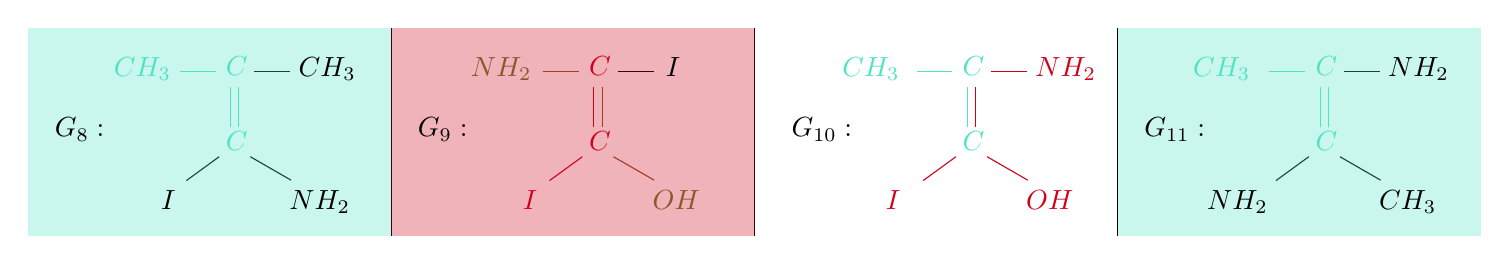
\begin{tikzpicture}[x=0.75pt,y=0.75pt,yscale=-1,xscale=1]
%uncomment if require: \path (0,300); %set diagram left start at 0, and has height of 300

%Straight Lines [id:da5237686775722785] 
\draw    (175,30) -- (175,130) ;
%Straight Lines [id:da28077840504722684] 
\draw    (350,30) -- (350,130) ;
%Straight Lines [id:da7851843321687619] 
\draw    (525,30) -- (525,130) ;
%Straight Lines [id:da846897062150809] 
\draw [color={rgb, 255:red, 80; green, 227; blue, 194 }  ,draw opacity=1 ][fill={rgb, 255:red, 74; green, 144; blue, 226 }  ,fill opacity=1 ]   (73,50.9) -- (90.29,50.9) ;
%Straight Lines [id:da5233570107936059] 
\draw    (109,50.9) -- (126.29,50.9) ;
%Straight Lines [id:da3570392511339686] 
\draw [color={rgb, 255:red, 80; green, 227; blue, 194 }  ,draw opacity=1 ]   (97.5,58.4) -- (97.5,77.4) ;
%Straight Lines [id:da5668461539599012] 
\draw [color={rgb, 255:red, 80; green, 227; blue, 194 }  ,draw opacity=1 ]   (101.5,58.4) -- (101.5,77.4) ;
%Straight Lines [id:da9335814717191053] 
\draw [color={rgb, 255:red, 0; green, 0; blue, 0 }  ,draw opacity=1 ]   (92,91.9) -- (76.2,103.41) ;
%Straight Lines [id:da4145258485980037] 
\draw    (126.61,103.2) -- (107,91.9) ;
%Straight Lines [id:da7798712844995945] 
\draw [color={rgb, 255:red, 139; green, 87; blue, 42 }  ,draw opacity=1 ]   (247.97,50.9) -- (265.26,50.9) ;
%Straight Lines [id:da6973389335797833] 
\draw    (283.97,50.9) -- (301.26,50.9) ;
%Straight Lines [id:da9972403694018135] 
\draw [color={rgb, 255:red, 208; green, 2; blue, 27 }  ,draw opacity=1 ]   (272.47,58.4) -- (272.47,77.4) ;
%Straight Lines [id:da23702841316511147] 
\draw [color={rgb, 255:red, 139; green, 87; blue, 42 }  ,draw opacity=1 ]   (276.47,58.4) -- (276.47,77.4) ;
%Straight Lines [id:da9764825376266975] 
\draw [color={rgb, 255:red, 208; green, 2; blue, 27 }  ,draw opacity=1 ]   (266.97,91.9) -- (251.17,103.41) ;
%Straight Lines [id:da8564770361796279] 
\draw [color={rgb, 255:red, 139; green, 87; blue, 42 }  ,draw opacity=1 ]   (301.57,103.2) -- (281.97,91.9) ;
%Straight Lines [id:da5805176197697994] 
\draw [color={rgb, 255:red, 80; green, 227; blue, 194 }  ,draw opacity=1 ]   (427.97,50.9) -- (445.26,50.9) ;
%Straight Lines [id:da25047126237464146] 
\draw [color={rgb, 255:red, 208; green, 2; blue, 27 }  ,draw opacity=1 ]   (463.97,50.9) -- (481.26,50.9) ;
%Straight Lines [id:da25124366061166703] 
\draw [color={rgb, 255:red, 80; green, 227; blue, 194 }  ,draw opacity=1 ]   (452.47,58.4) -- (452.47,77.4) ;
%Straight Lines [id:da894769536915182] 
\draw [color={rgb, 255:red, 208; green, 2; blue, 27 }  ,draw opacity=1 ]   (456.47,58.4) -- (456.47,77.4) ;
%Straight Lines [id:da5110832636857212] 
\draw [color={rgb, 255:red, 208; green, 2; blue, 27 }  ,draw opacity=1 ]   (446.97,91.9) -- (431.17,103.41) ;
%Straight Lines [id:da5912747311016606] 
\draw [color={rgb, 255:red, 208; green, 2; blue, 27 }  ,draw opacity=1 ]   (481.57,103.2) -- (461.97,91.9) ;
%Straight Lines [id:da3148852790405936] 
\draw [color={rgb, 255:red, 80; green, 227; blue, 194 }  ,draw opacity=1 ]   (597.97,50.9) -- (615.26,50.9) ;
%Straight Lines [id:da3387786073545902] 
\draw    (633.97,50.9) -- (651.26,50.9) ;
%Straight Lines [id:da07829059016645101] 
\draw [color={rgb, 255:red, 80; green, 227; blue, 194 }  ,draw opacity=1 ]   (622.47,58.4) -- (622.47,77.4) ;
%Straight Lines [id:da3415347439551548] 
\draw [color={rgb, 255:red, 80; green, 227; blue, 194 }  ,draw opacity=1 ]   (626.47,58.4) -- (626.47,77.4) ;
%Straight Lines [id:da6369740816090996] 
\draw    (616.97,91.9) -- (601.17,103.41) ;
%Straight Lines [id:da342082099953833] 
\draw    (651.57,103.2) -- (631.97,91.9) ;
%Shape: Rectangle [id:dp016671969434648437] 
\draw  [draw opacity=0][fill={rgb, 255:red, 80; green, 227; blue, 194 }  ,fill opacity=0.3 ] (0,30) -- (175,30) -- (175,130) -- (0,130) -- cycle ;
%Shape: Rectangle [id:dp5200027722915088] 
\draw  [draw opacity=0][fill={rgb, 255:red, 208; green, 2; blue, 27 }  ,fill opacity=0.3 ] (175,30) -- (350,30) -- (350,130) -- (175,130) -- cycle ;
%Shape: Rectangle [id:dp8291834814886794] 
\draw  [draw opacity=0][fill={rgb, 255:red, 80; green, 227; blue, 194 }  ,fill opacity=0.3 ] (525,30) -- (700,30) -- (700,130) -- (525,130) -- cycle ;

% Text Node
\draw (11.53,71.97) node [anchor=north west][inner sep=0.75pt]   [align=left] {$\displaystyle G_{8} :$};
% Text Node
\draw (40,42.7) node [anchor=north west][inner sep=0.75pt]  [color={rgb, 255:red, 80; green, 227; blue, 194 }  ,opacity=1 ] [align=left] {$\displaystyle CH_{3}$};
% Text Node
\draw (129,42.7) node [anchor=north west][inner sep=0.75pt]   [align=left] {$\displaystyle CH_{3}$};
% Text Node
\draw (94,42.3) node [anchor=north west][inner sep=0.75pt]  [color={rgb, 255:red, 80; green, 227; blue, 194 }  ,opacity=1 ] [align=left] {$\displaystyle C$};
% Text Node
\draw (62.73,106.77) node [anchor=north west][inner sep=0.75pt]   [align=left] {$\displaystyle I$};
% Text Node
\draw (94,78.38) node [anchor=north west][inner sep=0.75pt]  [color={rgb, 255:red, 80; green, 227; blue, 194 }  ,opacity=1 ] [align=left] {$\displaystyle C$};
% Text Node
\draw (124.61,106.8) node [anchor=north west][inner sep=0.75pt]   [align=left] {$\displaystyle NH_{2}$};
% Text Node
\draw (186.5,71.97) node [anchor=north west][inner sep=0.75pt]   [align=left] {$\displaystyle G_{9} :$};
% Text Node
\draw (211.97,42.7) node [anchor=north west][inner sep=0.75pt]  [color={rgb, 255:red, 139; green, 87; blue, 42 }  ,opacity=1 ] [align=left] {$\displaystyle NH_{2}$};
% Text Node
\draw (305.97,42.7) node [anchor=north west][inner sep=0.75pt]   [align=left] {$\displaystyle I$};
% Text Node
\draw (268.97,42.3) node [anchor=north west][inner sep=0.75pt]  [color={rgb, 255:red, 208; green, 2; blue, 27 }  ,opacity=1 ] [align=left] {$\displaystyle C$};
% Text Node
\draw (237,106.77) node [anchor=north west][inner sep=0.75pt]  [color={rgb, 255:red, 208; green, 2; blue, 27 }  ,opacity=1 ] [align=left] {$\displaystyle I$};
% Text Node
\draw (268.97,78.38) node [anchor=north west][inner sep=0.75pt]  [color={rgb, 255:red, 208; green, 2; blue, 27 }  ,opacity=1 ] [align=left] {$\displaystyle C$};
% Text Node
\draw (299.57,106.8) node [anchor=north west][inner sep=0.75pt]  [color={rgb, 255:red, 139; green, 87; blue, 42 }  ,opacity=1 ] [align=left] {$\displaystyle OH$};
% Text Node
\draw (366.5,71.97) node [anchor=north west][inner sep=0.75pt]   [align=left] {$\displaystyle G_{10} :$};
% Text Node
\draw (390.97,42.8) node [anchor=north west][inner sep=0.75pt]  [color={rgb, 255:red, 80; green, 227; blue, 194 }  ,opacity=1 ] [align=left] {$\displaystyle CH_{3}$};
% Text Node
\draw (483.97,42.7) node [anchor=north west][inner sep=0.75pt]  [color={rgb, 255:red, 208; green, 2; blue, 27 }  ,opacity=1 ] [align=left] {$\displaystyle NH_{2}$};
% Text Node
\draw (448.97,42.3) node [anchor=north west][inner sep=0.75pt]  [color={rgb, 255:red, 80; green, 227; blue, 194 }  ,opacity=1 ] [align=left] {$\displaystyle C$};
% Text Node
\draw (412,106.77) node [anchor=north west][inner sep=0.75pt]  [color={rgb, 255:red, 208; green, 2; blue, 27 }  ,opacity=1 ] [align=left] {$\displaystyle I$};
% Text Node
\draw (448.97,78.38) node [anchor=north west][inner sep=0.75pt]  [color={rgb, 255:red, 80; green, 227; blue, 194 }  ,opacity=1 ] [align=left] {$\displaystyle C$};
% Text Node
\draw (479.57,106.8) node [anchor=north west][inner sep=0.75pt]  [color={rgb, 255:red, 208; green, 2; blue, 27 }  ,opacity=1 ] [align=left] {$\displaystyle OH$};
% Text Node
\draw (536.5,71.97) node [anchor=north west][inner sep=0.75pt]   [align=left] {$\displaystyle G_{11} :$};
% Text Node
\draw (559.97,42.7) node [anchor=north west][inner sep=0.75pt]  [color={rgb, 255:red, 80; green, 227; blue, 194 }  ,opacity=1 ] [align=left] {$\displaystyle CH_{3}$};
% Text Node
\draw (653.97,42.7) node [anchor=north west][inner sep=0.75pt]   [align=left] {$\displaystyle NH_{2}$};
% Text Node
\draw (618.97,42.3) node [anchor=north west][inner sep=0.75pt]  [color={rgb, 255:red, 80; green, 227; blue, 194 }  ,opacity=1 ] [align=left] {$\displaystyle C$};
% Text Node
\draw (566.7,106.77) node [anchor=north west][inner sep=0.75pt]   [align=left] {$\displaystyle NH_{2}$};
% Text Node
\draw (618.97,78.38) node [anchor=north west][inner sep=0.75pt]  [color={rgb, 255:red, 80; green, 227; blue, 194 }  ,opacity=1 ] [align=left] {$\displaystyle C$};
% Text Node
\draw (649.57,106.8) node [anchor=north west][inner sep=0.75pt]   [align=left] {$\displaystyle CH_{3}$};


\end{tikzpicture}
\end{figure}
\begin{itemize}
  \item Object $G_8$ is classified positively, because:
  \[
      H^+ \sqsubseteq G_8^\diamond, \ H^- \not\sqsubseteq G_8^\diamond
  \]
  \item Object $G_9$ is classified negatively, because:
  \[
    H^- \sqsubseteq G_9^\diamond, \ H^+ \not\sqsubseteq G_9^\diamond
  \]
  \item Object $G_{10}$ is classified contradictory, because:
  \[
    H^-, H^+ \sqsubseteq G_{10}^\diamond
  \]
  \item Object $G_{11}$ is classified positively, because:
  \[
    H^+ \sqsubseteq G_{11}^\diamond, \ H^- \not\sqsubseteq G_{11}^\diamond
  \]
\end{itemize}
\end{solution}
\end{document}